
%% bare_jrnl_compsoc.tex
%% V1.3
%% 2007/01/11
%% by Michael Shell
%% See:
%% http://www.michaelshell.org/
%% for current contact information.
%%
%% This is a skeleton file demonstrating the use of IEEEtran.cls
%% (requires IEEEtran.cls version 1.7 or later) with an IEEE Computer
%% Society journal paper.
%%
%% Support sites:
%% http://www.michaelshell.org/tex/ieeetran/
%% http://www.ctan.org/tex-archive/macros/latex/contrib/IEEEtran/
%% and
%% http://www.ieee.org/

%%*************************************************************************
%% Legal Notice:
%% This code is offered as-is without any warranty either expressed or
%% implied; without even the implied warranty of MERCHANTABILITY or
%% FITNESS FOR A PARTICULAR PURPOSE!
%% User assumes all risk.
%% In no event shall IEEE or any contributor to this code be liable for
%% any damages or losses, including, but not limited to, incidental,
%% consequential, or any other damages, resulting from the use or misuse
%% of any information contained here.
%%
%% All comments are the opinions of their respective authors and are not
%% necessarily endorsed by the IEEE.
%%
%% This work is distributed under the LaTeX Project Public License (LPPL)
%% ( http://www.latex-project.org/ ) version 1.3, and may be freely used,
%% distributed and modified. A copy of the LPPL, version 1.3, is included
%% in the base LaTeX documentation of all distributions of LaTeX released
%% 2003/12/01 or later.
%% Retain all contribution notices and credits.
%% ** Modified files should be clearly indicated as such, including  **
%% ** renaming them and changing author support contact information. **
%%
%% File list of work: IEEEtran.cls, IEEEtran_HOWTO.pdf, bare_adv.tex,
%%                    bare_conf.tex, bare_jrnl.tex, bare_jrnl_compsoc.tex
%%*************************************************************************

% *** Authors should verify (and, if needed, correct) their LaTeX system  ***
% *** with the testflow diagnostic prior to trusting their LaTeX platform ***
% *** with production work. IEEE's font choices can trigger bugs that do  ***
% *** not appear when using other class files.                            ***
% The testflow support page is at:
% http://www.michaelshell.org/tex/testflow/




% Note that the a4paper option is mainly intended so that authors in
% countries using A4 can easily print to A4 and see how their papers will
% look in print - the typesetting of the document will not typically be
% affected with changes in paper size (but the bottom and side margins will).
% Use the testflow package mentioned above to verify correct handling of
% both paper sizes by the user's LaTeX system.
%
% Also note that the "draftcls" or "draftclsnofoot", not "draft", option
% should be used if it is desired that the figures are to be displayed in
% draft mode.
%
% The Computer Society usually requires 10pt for submissions.
%

\documentclass[10pt,journal,cspaper,compsoc]{IEEEtran}
\usepackage{graphicx}
\usepackage{amsthm}
\usepackage{algpseudocode}
\usepackage{algorithm}
\usepackage{amsmath}

\algrenewcommand{\algorithmicrequire}{\textbf{Input:}}
\algrenewcommand{\algorithmicensure}{\textbf{Output:}}
\renewcommand{\algorithmicforall}{\textbf{for each}}
%
% If IEEEtran.cls has not been installed into the LaTeX system files,
% manually specify the path to it like:
% \documentclass[12pt,journal,compsoc]{../sty/IEEEtran}





% Some very useful LaTeX packages include:
% (uncomment the ones you want to load)


% *** MISC UTILITY PACKAGES ***
%
%\usepackage{ifpdf}
% Heiko Oberdiek's ifpdf.sty is very useful if you need conditional
% compilation based on whether the output is pdf or dvi.
% usage:
% \ifpdf
%   % pdf code
% \else
%   % dvi code
% \fi
% The latest version of ifpdf.sty can be obtained from:
% http://www.ctan.org/tex-archive/macros/latex/contrib/oberdiek/
% Also, note that IEEEtran.cls V1.7 and later provides a builtin
% \ifCLASSINFOpdf conditional that works the same way.
% When switching from latex to pdflatex and vice-versa, the compiler may
% have to be run twice to clear warning/error messages.






% *** CITATION PACKAGES ***
%
\ifCLASSOPTIONcompsoc
  % IEEE Computer Society needs nocompress option
  % requires cite.sty v4.0 or later (November 2003)
  % \usepackage[nocompress]{cite}
\else
  % normal IEEE
  % \usepackage{cite}
\fi
% cite.sty was written by Donald Arseneau
% V1.6 and later of IEEEtran pre-defines the format of the cite.sty package
% \cite{} output to follow that of IEEE. Loading the cite package will
% result in citation numbers being automatically sorted and properly
% "compressed/ranged". e.g., [1], [9], [2], [7], [5], [6] without using
% cite.sty will become [1], [2], [5]--[7], [9] using cite.sty. cite.sty's
% \cite will automatically add leading space, if needed. Use cite.sty's
% noadjust option (cite.sty V3.8 and later) if you want to turn this off.
% cite.sty is already installed on most LaTeX systems. Be sure and use
% version 4.0 (2003-05-27) and later if using hyperref.sty. cite.sty does
% not currently provide for hyperlinked citations.
% The latest version can be obtained at:
% http://www.ctan.org/tex-archive/macros/latex/contrib/cite/
% The documentation is contained in the cite.sty file itself.
%
% Note that some packages require special options to format as the Computer
% Society requires. In particular, Computer Society  papers do not use
% compressed citation ranges as is done in typical IEEE papers
% (e.g., [1]-[4]). Instead, they list every citation separately in order
% (e.g., [1], [2], [3], [4]). To get the latter we need to load the cite
% package with the nocompress option which is supported by cite.sty v4.0
% and later. Note also the use of a CLASSOPTION conditional provided by
% IEEEtran.cls V1.7 and later.





% *** GRAPHICS RELATED PACKAGES ***
%
\ifCLASSINFOpdf
  % \usepackage[pdftex]{graphicx}
  % declare the path(s) where your graphic files are
  % \graphicspath{{../pdf/}{../jpeg/}}
  % and their extensions so you won't have to specify these with
  % every instance of \includegraphics
  % \DeclareGraphicsExtensions{.pdf,.jpeg,.png}
\else
  % or other class option (dvipsone, dvipdf, if not using dvips). graphicx
  % will default to the driver specified in the system graphics.cfg if no
  % driver is specified.
  % \usepackage[dvips]{graphicx}
  % declare the path(s) where your graphic files are
  % \graphicspath{{../eps/}}
  % and their extensions so you won't have to specify these with
  % every instance of \includegraphics
  % \DeclareGraphicsExtensions{.eps}
\fi
% graphicx was written by David Carlisle and Sebastian Rahtz. It is
% required if you want graphics, photos, etc. graphicx.sty is already
% installed on most LaTeX systems. The latest version and documentation can
% be obtained at:
% http://www.ctan.org/tex-archive/macros/latex/required/graphics/
% Another good source of documentation is "Using Imported Graphics in
% LaTeX2e" by Keith Reckdahl which can be found as epslatex.ps or
% epslatex.pdf at: http://www.ctan.org/tex-archive/info/
%
% latex, and pdflatex in dvi mode, support graphics in encapsulated
% postscript (.eps) format. pdflatex in pdf mode supports graphics
% in .pdf, .jpeg, .png and .mps (metapost) formats. Users should ensure
% that all non-photo figures use a vector format (.eps, .pdf, .mps) and
% not a bitmapped formats (.jpeg, .png). IEEE frowns on bitmapped formats
% which can result in "jaggedy"/blurry rendering of lines and letters as
% well as large increases in file sizes.
%
% You can find documentation about the pdfTeX application at:
% http://www.tug.org/applications/pdftex





% *** MATH PACKAGES ***
%
%\usepackage[cmex10]{amsmath}
% A popular package from the American Mathematical Society that provides
% many useful and powerful commands for dealing with mathematics. If using
% it, be sure to load this package with the cmex10 option to ensure that
% only type 1 fonts will utilized at all point sizes. Without this option,
% it is possible that some math symbols, particularly those within
% footnotes, will be rendered in bitmap form which will result in a
% document that can not be IEEE Xplore compliant!
%
% Also, note that the amsmath package sets \interdisplaylinepenalty to 10000
% thus preventing page breaks from occurring within multiline equations. Use:
%\interdisplaylinepenalty=2500
% after loading amsmath to restore such page breaks as IEEEtran.cls normally
% does. amsmath.sty is already installed on most LaTeX systems. The latest
% version and documentation can be obtained at:
% http://www.ctan.org/tex-archive/macros/latex/required/amslatex/math/





% *** SPECIALIZED LIST PACKAGES ***
%
%\usepackage{algorithmic}
% algorithmic.sty was written by Peter Williams and Rogerio Brito.
% This package provides an algorithmic environment fo describing algorithms.
% You can use the algorithmic environment in-text or within a figure
% environment to provide for a floating algorithm. Do NOT use the algorithm
% floating environment provided by algorithm.sty (by the same authors) or
% algorithm2e.sty (by Christophe Fiorio) as IEEE does not use dedicated
% algorithm float types and packages that provide these will not provide
% correct IEEE style captions. The latest version and documentation of
% algorithmic.sty can be obtained at:
% http://www.ctan.org/tex-archive/macros/latex/contrib/algorithms/
% There is also a support site at:
% http://algorithms.berlios.de/index.html
% Also of interest may be the (relatively newer and more customizable)
% algorithmicx.sty package by Szasz Janos:
% http://www.ctan.org/tex-archive/macros/latex/contrib/algorithmicx/




% *** ALIGNMENT PACKAGES ***
%
%\usepackage{array}
% Frank Mittelbach's and David Carlisle's array.sty patches and improves
% the standard LaTeX2e array and tabular environments to provide better
% appearance and additional user controls. As the default LaTeX2e table
% generation code is lacking to the point of almost being broken with
% respect to the quality of the end results, all users are strongly
% advised to use an enhanced (at the very least that provided by array.sty)
% set of table tools. array.sty is already installed on most systems. The
% latest version and documentation can be obtained at:
% http://www.ctan.org/tex-archive/macros/latex/required/tools/


%\usepackage{mdwmath}
%\usepackage{mdwtab}
% Also highly recommended is Mark Wooding's extremely powerful MDW tools,
% especially mdwmath.sty and mdwtab.sty which are used to format equations
% and tables, respectively. The MDWtools set is already installed on most
% LaTeX systems. The lastest version and documentation is available at:
% http://www.ctan.org/tex-archive/macros/latex/contrib/mdwtools/


% IEEEtran contains the IEEEeqnarray family of commands that can be used to
% generate multiline equations as well as matrices, tables, etc., of high
% quality.


%\usepackage{eqparbox}
% Also of notable interest is Scott Pakin's eqparbox package for creating
% (automatically sized) equal width boxes - aka "natural width parboxes".
% Available at:
% http://www.ctan.org/tex-archive/macros/latex/contrib/eqparbox/





% *** SUBFIGURE PACKAGES ***
%\ifCLASSOPTIONcompsoc
%\usepackage[tight,normalsize,sf,SF]{subfigure}
%\else
%\usepackage[tight,footnotesize]{subfigure}
%\fi
% subfigure.sty was written by Steven Douglas Cochran. This package makes it
% easy to put subfigures in your figures. e.g., "Figure 1a and 1b". For IEEE
% work, it is a good idea to load it with the tight package option to reduce
% the amount of white space around the subfigures. Computer Society papers
% use a larger font and \sffamily font for their captions, hence the
% additional options needed under compsoc mode. subfigure.sty is already
% installed on most LaTeX systems. The latest version and documentation can
% be obtained at:
% http://www.ctan.org/tex-archive/obsolete/macros/latex/contrib/subfigure/
% subfigure.sty has been superceeded by subfig.sty.


%\ifCLASSOPTIONcompsoc
%  \usepackage[caption=false]{caption}
%  \usepackage[font=normalsize,labelfont=sf,textfont=sf]{subfig}
%\else
%  \usepackage[caption=false]{caption}
%  \usepackage[font=footnotesize]{subfig}
%\fi
% subfig.sty, also written by Steven Douglas Cochran, is the modern
% replacement for subfigure.sty. However, subfig.sty requires and
% automatically loads Axel Sommerfeldt's caption.sty which will override
% IEEEtran.cls handling of captions and this will result in nonIEEE style
% figure/table captions. To prevent this problem, be sure and preload
% caption.sty with its "caption=false" package option. This is will preserve
% IEEEtran.cls handing of captions. Version 1.3 (2005/06/28) and later
% (recommended due to many improvements over 1.2) of subfig.sty supports
% the caption=false option directly:
%\ifCLASSOPTIONcompsoc
%  \usepackage[caption=false,font=normalsize,labelfont=sf,textfont=sf]{subfig}
%\else
%  \usepackage[caption=false,font=footnotesize]{subfig}
%\fi
%
% The latest version and documentation can be obtained at:
% http://www.ctan.org/tex-archive/macros/latex/contrib/subfig/
% The latest version and documentation of caption.sty can be obtained at:
% http://www.ctan.org/tex-archive/macros/latex/contrib/caption/




% *** FLOAT PACKAGES ***
%
%\usepackage{fixltx2e}
% fixltx2e, the successor to the earlier fix2col.sty, was written by
% Frank Mittelbach and David Carlisle. This package corrects a few problems
% in the LaTeX2e kernel, the most notable of which is that in current
% LaTeX2e releases, the ordering of single and double column floats is not
% guaranteed to be preserved. Thus, an unpatched LaTeX2e can allow a
% single column figure to be placed prior to an earlier double column
% figure. The latest version and documentation can be found at:
% http://www.ctan.org/tex-archive/macros/latex/base/



%\usepackage{stfloats}
% stfloats.sty was written by Sigitas Tolusis. This package gives LaTeX2e
% the ability to do double column floats at the bottom of the page as well
% as the top. (e.g., "\begin{figure*}[!b]" is not normally possible in
% LaTeX2e). It also provides a command:
%\fnbelowfloat
% to enable the placement of footnotes below bottom floats (the standard
% LaTeX2e kernel puts them above bottom floats). This is an invasive package
% which rewrites many portions of the LaTeX2e float routines. It may not work
% with other packages that modify the LaTeX2e float routines. The latest
% version and documentation can be obtained at:
% http://www.ctan.org/tex-archive/macros/latex/contrib/sttools/
% Documentation is contained in the stfloats.sty comments as well as in the
% presfull.pdf file. Do not use the stfloats baselinefloat ability as IEEE
% does not allow \baselineskip to stretch. Authors submitting work to the
% IEEE should note that IEEE rarely uses double column equations and
% that authors should try to avoid such use. Do not be tempted to use the
% cuted.sty or midfloat.sty packages (also by Sigitas Tolusis) as IEEE does
% not format its papers in such ways.




%\ifCLASSOPTIONcaptionsoff
%  \usepackage[nomarkers]{endfloat}
% \let\MYoriglatexcaption\caption
% \renewcommand{\caption}[2][\relax]{\MYoriglatexcaption[#2]{#2}}
%\fi
% endfloat.sty was written by James Darrell McCauley and Jeff Goldberg.
% This package may be useful when used in conjunction with IEEEtran.cls'
% captionsoff option. Some IEEE journals/societies require that submissions
% have lists of figures/tables at the end of the paper and that
% figures/tables without any captions are placed on a page by themselves at
% the end of the document. If needed, the draftcls IEEEtran class option or
% \CLASSINPUTbaselinestretch interface can be used to increase the line
% spacing as well. Be sure and use the nomarkers option of endfloat to
% prevent endfloat from "marking" where the figures would have been placed
% in the text. The two hack lines of code above are a slight modification of
% that suggested by in the endfloat docs (section 8.3.1) to ensure that
% the full captions always appear in the list of figures/tables - even if
% the user used the short optional argument of \caption[]{}.
% IEEE papers do not typically make use of \caption[]'s optional argument,
% so this should not be an issue. A similar trick can be used to disable
% captions of packages such as subfig.sty that lack options to turn off
% the subcaptions:
% For subfig.sty:
% \let\MYorigsubfloat\subfloat
% \renewcommand{\subfloat}[2][\relax]{\MYorigsubfloat[]{#2}}
% For subfigure.sty:
% \let\MYorigsubfigure\subfigure
% \renewcommand{\subfigure}[2][\relax]{\MYorigsubfigure[]{#2}}
% However, the above trick will not work if both optional arguments of
% the \subfloat/subfig command are used. Furthermore, there needs to be a
% description of each subfigure *somewhere* and endfloat does not add
% subfigure captions to its list of figures. Thus, the best approach is to
% avoid the use of subfigure captions (many IEEE journals avoid them anyway)
% and instead reference/explain all the subfigures within the main caption.
% The latest version of endfloat.sty and its documentation can obtained at:
% http://www.ctan.org/tex-archive/macros/latex/contrib/endfloat/
%
% The IEEEtran \ifCLASSOPTIONcaptionsoff conditional can also be used
% later in the document, say, to conditionally put the References on a
% page by themselves.




% *** PDF, URL AND HYPERLINK PACKAGES ***
%
%\usepackage{url}
% url.sty was written by Donald Arseneau. It provides better support for
% handling and breaking URLs. url.sty is already installed on most LaTeX
% systems. The latest version can be obtained at:
% http://www.ctan.org/tex-archive/macros/latex/contrib/misc/
% Read the url.sty source comments for usage information. Basically,
% \url{my_url_here}.





% *** Do not adjust lengths that control margins, column widths, etc. ***
% *** Do not use packages that alter fonts (such as pslatex).         ***
% There should be no need to do such things with IEEEtran.cls V1.6 and later.
% (Unless specifically asked to do so by the journal or conference you plan
% to submit to, of course. )


% correct bad hyphenation here
\hyphenation{op-tical net-works semi-conduc-tor}


\begin{document}
%
% paper title
% can use linebreaks \\ within to get better formatting as desired
\title{A more efficient and effective MFS Identification method}
%
%
% author names and IEEE memberships
% note positions of commas and nonbreaking spaces ( ~ ) LaTeX will not break
% a structure at a ~ so this keeps an author's name from being broken across
% two lines.
% use \thanks{} to gain access to the first footnote area
% a separate \thanks must be used for each paragraph as LaTeX2e's \thanks
% was not built to handle multiple paragraphs
%
%
%\IEEEcompsocitemizethanks is a special \thanks that produces the bulleted
% lists the Computer Society journals use for "first footnote" author
% affiliations. Use \IEEEcompsocthanksitem which works much like \item
% for each affiliation group. When not in compsoc mode,
% \IEEEcompsocitemizethanks becomes like \thanks and
% \IEEEcompsocthanksitem becomes a line break with idention. This
% facilitates dual compilation, although admittedly the differences in the
% desired content of \author between the different types of papers makes a
% one-size-fits-all approach a daunting prospect. For instance, compsoc
% journal papers have the author affiliations above the "Manuscript
% received ..."  text while in non-compsoc journals this is reversed. Sigh.

\author{Xintao~Niu,~
        Changhai~Nie,~\IEEEmembership{Member,~IEEE,}
        and~~% <-this % stops a space
\IEEEcompsocitemizethanks{\IEEEcompsocthanksitem Xintao Niu and Changhai Nie are with the State Key Laboratory for Novel Software Technology, Nanjing University, China, 210023. \protect\\
% note need leading \protect in front of \\ to get a newline within \thanks as
% \\ is fragile and will error, could use \hfil\break instead.
E-mail: niuxintao@gmail.com, changhainie@nju.edu.cn
% note need leading \protect in front of \\ to get a newline within \thanks as
% \\ is fragile and will error, could use \hfil\break instead.
\IEEEcompsocthanksitem Hareton Leung is with Department of computing, Hong Kong Polytechnic University, Kowloon, Hong Kong. \protect\\
  E-mail: hareton.leung@polyu.edu.hk
\IEEEcompsocthanksitem Jeff Y. Lei is with Department of Computer Science and Engineering, The University of Texas at Arlington, Arlington, Texas. \protect\\
  E-mail: ylei@cse.uta.edu
\IEEEcompsocthanksitem Xiaoyin Wang is with Department of Computer Science, University of Texas at San Antonio. \protect\\
  E-mail: Xiaoyin.Wang@utsa.edu}% <-this % stops an unwanted space
\thanks{Manuscript received April 19, 2005; revised September 17, 2014.}}

% note the % following the last \IEEEmembership and also \thanks -
% these prevent an unwanted space from occurring between the last author name
% and the end of the author line. i.e., if you had this:
%
% \author{....lastname \thanks{...} \thanks{...} }
%                     ^------------^------------^----Do not want these spaces!
%
% a space would be appended to the last name and could cause every name on that
% line to be shifted left slightly. This is one of those "LaTeX things". For
% instance, "\textbf{A} \textbf{B}" will typeset as "A B" not "AB". To get
% "AB" then you have to do: "\textbf{A}\textbf{B}"
% \thanks is no different in this regard, so shield the last } of each \thanks
% that ends a line with a % and do not let a space in before the next \thanks.
% Spaces after \IEEEmembership other than the last one are OK (and needed) as
% you are supposed to have spaces between the names. For what it is worth,
% this is a minor point as most people would not even notice if the said evil
% space somehow managed to creep in.



% The paper headers
\markboth{Journal of \LaTeX\ Class Files,~Vol.~6, No.~1, January~2007}%
{Shell \MakeLowercase{\textit{et al.}}: Bare Demo of IEEEtran.cls for Computer Society Journals}
% The only time the second header will appear is for the odd numbered pages
% after the title page when using the twoside option.
%
% *** Note that you probably will NOT want to include the author's ***
% *** name in the headers of peer review papers.                   ***
% You can use \ifCLASSOPTIONpeerreview for conditional compilation here if
% you desire.



% The publisher's ID mark at the bottom of the page is less important with
% Computer Society journal papers as those publications place the marks
% outside of the main text columns and, therefore, unlike regular IEEE
% journals, the available text space is not reduced by their presence.
% If you want to put a publisher's ID mark on the page you can do it like
% this:
%\IEEEpubid{0000--0000/00\$00.00~\copyright~2007 IEEE}
% or like this to get the Computer Society new two part style.
%\IEEEpubid{\makebox[\columnwidth]{\hfill 0000--0000/00/\$00.00~\copyright~2007 IEEE}%
%\hspace{\columnsep}\makebox[\columnwidth]{Published by the IEEE Computer Society\hfill}}
% Remember, if you use this you must call \IEEEpubidadjcol in the second
% column for its text to clear the IEEEpubid mark (Computer Society jorunal
% papers don't need this extra clearance.)




% for Computer Society papers, we must declare the abstract and index terms
% PRIOR to the title within the \IEEEcompsoctitleabstractindextext IEEEtran
% command as these need to go into the title area created by \maketitle.
\IEEEcompsoctitleabstractindextext{%
\begin{abstract}
%\boldmath
Combinatorial testing (CT) aims to detect the failures which are triggered by the interactions of various factors that can influence the behaviour of the system, such as input parameters, configuration options, and specific events. Many studies in CT focus on designing a elaborate test suite (called covering array) to reveal such failures. When a interaction failure is detected, it is desired to identify the root cause of that failure, i.e., the failure-inducing interactions. Although covering array can assist testers to systemically check each possible factor interactions (without masking effects), however, it provides weak support to locate the failure-inducing interactions. Hence, more auxiliary information are needed to filter out those failure-irrelevant interactions and obtain the failure-inducing ones. Recently some elementary researches are proposed to handle the failure-inducing interaction identification problem. However, some issues, such as unable to identify multiple failure-inducing interactions, and generating too many additional test cases, negatively influence the applicability of these approaches. In this paper, we propose a novel failure-inducing identification approach which aims to handle those issues. The key of our approach is to search for a proper factor interaction at each iteration to check whether it is failure-inducing or not until all the interactions in a failing test cases are checked. To reach this target, we maintain two data structures to guide the selection, i.e., CMINFS(represent for candidate minimal faulty schemas) and CMAXHS(represent for candidate maximal healthy schemas). With these two data set, an optimal interaction can be selected to check so that we can reduce as many additional test cases as possible, as well as not ignore any unchecked-interactions, e.g., the interactions with large number of factors. Our approach will repeat updating the interactions in these two set after a interaction is checked. Moreover, we conduct empirical studies on both widely-used real highly-configurable software systems and synthetic softwares. Results showed that our approach obtained a higher quality at the failure-inducing interaction identification, while just needed a smaller number of additional test cases.


%at each iteraction.  Our approach works by checking each possible factor interaction in a failing test case, we check. With this ,  Our approach can ensure that each possible interaction in a failing test case is checked or onr. As a consequent, we can avoid many, such as mutliple, overlapping, hihger degree.

%can get an efficient performance when identifying the failure-inducing schemas compared to prior works. Also we make an improvement on the approach to better handle the case where additional failure-inducing schemas may be introduced by newly generated test configurations.
%
%Moreover, we conduct empirical studies on both widely-used real highly-configurable software systems and simulated toy softwares.The results shows that the failure-inducing schemas do exist in software and our approach can identify them more effectively and efficiently than other works.

%To how to characterize the interaction faults. Hence some studies are proposed to support a further diagnosis approach. From those studies, OFOT is simple.   Although covering array is proven to be effective to detect the interaction failure in the software, however, it is still far from to locate the failure-inducing interactions. Some studies
% It is a large testing space, when exhaustive is impossible. Combinatorial testing technique is a relief to this problem by design a small test suite to cover the interactions not exceed to a strength t. Nevertheless, most studies in CT focus on the generating suite, Thus, we can't determine which even when we detect them for there are many candidates interactions. publish. The behaviour of modern softwares is influenced by many factors. These factors can be the inputs of the system, configuration options , user events and so on. It is a big pressure to the testing when the factors increase rapidly and the interactions between these factors. It is common that the software under test(SUT) fails during testing under some specific test configurations(we called failing configurations) and passes under the others. For these failing configurations,in the most general case,not all the options in this configuration is related to the failures. It is desirable to identify the specific options responsible for the failures,i.e., failure-inducing schemas,as by doing this it can reduce the debugging effort.
%
%Combinatorial testing(CT) can effectively detect the errors in SUT which are triggered by interactions of options.However, it provide weak support for identifying them. In this paper, we propose an efficient approach which can aids the CT to locate them.Through using the notions of CMINFS(represent for candidate minimal faulty schemas) and CMAXHS(represent for candidate maximal healthy schemas), our approach can get an efficient performance when identifying the failure-inducing schemas compared to our prior work.Also we make an improvement on the approach to better handle the case where additional failure-inducing schemas may be introduced by newly generated test configurations.
%
%Moreover, we conduct empirical studies on both widely-used real highly-configurable software systems and simulated toy softwares.The results shows that the failure-inducing schemas do exist in software and our approach can identify them more effectively and efficiently than other works.
\end{abstract}
% IEEEtran.cls defaults to using nonbold math in the Abstract.
% This preserves the distinction between vectors and scalars. However,
% if the journal you are submitting to favors bold math in the abstract,
% then you can use LaTeX's standard command \boldmath at the very start
% of the abstract to achieve this. Many IEEE journals frown on math
% in the abstract anyway. In particular, the Computer Society does
% not want either math or citations to appear in the abstract.

% Note that keywords are not normally used for peer review papers.
\begin{keywords}
failure-inducing interactions, fault location, debugging aids, combinatorial testing
\end{keywords}}


% make the title area
\maketitle


% To allow for easy dual compilation without having to reenter the
% abstract/keywords data, the \IEEEcompsoctitleabstractindextext text will
% not be used in maketitle, but will appear (i.e., to be "transported")
% here as \IEEEdisplaynotcompsoctitleabstractindextext when compsoc mode
% is not selected <OR> if conference mode is selected - because compsoc
% conference papers position the abstract like regular (non-compsoc)
% papers do!
\IEEEdisplaynotcompsoctitleabstractindextext
% \IEEEdisplaynotcompsoctitleabstractindextext has no effect when using
% compsoc under a non-conference mode.


% For peer review papers, you can put extra information on the cover
% page as needed:
% \ifCLASSOPTIONpeerreview
% \begin{center} \bfseries EDICS Category: 3-BBND \end{center}
% \fi
%
% For peerreview papers, this IEEEtran command inserts a page break and
% creates the second title. It will be ignored for other modes.
\IEEEpeerreviewmaketitle



\section{Introduction}\label{sec:intro}
% Computer Society journal papers do something a tad strange with the very
% first section heading (almost always called "Introduction"). They place it
% ABOVE the main text! IEEEtran.cls currently does not do this for you.
% However, You can achieve this effect by making LaTeX jump through some
% hoops via something like:
%
%\ifCLASSOPTIONcompsoc
%  \noindent\raisebox{2\baselineskip}[0pt][0pt]%
%  {\parbox{\columnwidth}{\section{Introduction}\label{sec:introduction}%
%  \global\everypar=\everypar}}%
%  \vspace{-1\baselineskip}\vspace{-\parskip}\par
%\else
%  \section{Introduction}\label{sec:introduction}\par
%\fi
%
% Admittedly, this is a hack and may well be fragile, but seems to do the
% trick for me. Note the need to keep any \label that may be used right
% after \section in the above as the hack puts \section within a raised box.



% The very first letter is a 2 line initial drop letter followed
% by the rest of the first word in caps (small caps for compsoc).
%
% form to use if the first word consists of a single letter:
% \IEEEPARstart{A}{demo} file is ....
%
% form to use if you need the single drop letter followed by
% normal text (unknown if ever used by IEEE):
% \IEEEPARstart{A}{}demo file is ....
%
% Some journals put the first two words in caps:
% \IEEEPARstart{T}{his demo} file is ....
%
% Here we have the typical use of a "T" for an initial drop letter
% and "HIS" in caps to complete the first word.
\IEEEPARstart{T}he behavior of modern software are affected by many factors, such as input parameters, configuration options, and specific events. To test such software system is challenging, as in theory we should test all the possible interaction of these factors to ensure the correctness of the System Under Test (SUT)\cite{song2012itree}. When the number of factors is large, the interactions that are needed to check increase exponentially. Hence it is, if possible, not practical to conduct such exhaustive testing. Combinatorial testing (CT) is a promising solution to handle the combinatorial explosion problem. Instead of testing all the possible interactions in a system, it focus on checking those interactions with number of involved factors no more than a prior number. Commonly when applying CT, a elaborate test suite (called covering array) will be generated to cover the valid interaction that needs to be checked. Although covering array is effective and efficient as a test suite, however, it provides weak support to distinguish the failure-inducing interactions from all the interactions.
%This is mainly because  In other word, it is far from with covering array alone.
%which is not feasible in practice. Combinatorial testing technique can handle this problem well. It design a relatively small test suite from the configuration spaces to test the SUT and can ensure to cover all the interactions of option values which not exceed t. When we find some configurations fail in this test suite, which means this suite detect some interaction fault, what we want to know next is to identify which specific interaction options and its values are the cause of these failures. To our best know, combinatorial testing provide week support to identify them.
% You must have at least 2 lines in the paragraph with the drop letter
% (should never be an issue)

Consider the following example \cite{bach2004pairwise}, Table \ref{MS_word} presents a pair-wise covering array for testing an MS-Word application in which we want to examine various pair-wise interactions of options for `Highlight', `Status Bar', `Bookmarks' and `Smart tags'. Assume the third test case failed. We can get five pair-wise suspicious interactions that may be responsible for this failure. They are respectively (Highlight: Off, Status Bar: On), (Highlight: Off, Bookmarks: Off), (Highlight: Off, Smart tags: Off), (Status Bar: On, Bookmarks: Off), (Status Bar: On, Smart tags: Off),  and (Bookmarks: Off, Smart tags: Off). Without additional information, it is difficult to figure out the specific interactions in this suspicious set that caused the failure. In fact, considering that the interactions consist of other number of factors could also be failure-inducing interactions, e.g., (Highlight: Off) and (Highlight: Off, Status Bar: On, Smart tags: Off), the problem becomes more complicated. Generally, to definitely determine the failure-inducing interactions in a failing test case of \emph{n} factors, we need to check all the $2^n - 1$ interactions in this test case, which is not possible when \emph{n} is a large number.

\begin{table}
\caption{MS word example} \centering
  \label{MS_word}
  \setlength{\tabcolsep}{3pt}
  \begin{tabular}{c|cccc|c}
id& \emph{Highlight} & \emph{Status bar} & \emph{Bookmarks}& \emph{Smart tags} & \bfseries{Outcome} \\\hline
1& On & On & On& On & PASS\\ \hline
2& Off & Off & On & On & PASS\\ \hline
3&Off&	On&	Off&Off & Fail\\ \hline
4&On & Off & Off &On&  PASS\\ \hline
5&On & Off &On & Off&  PASS\\ \hline
  \end{tabular}
\end{table}

To address this problem, prior work \cite{nie2011minimal} specifically studied the properties of the failure-inducing interactions in SUT, based on which additional test cases were generated to identify them. Other approaches to identify the failure-inducing interactions in SUT include building a tree model \cite{yilmaz2006covering}, adaptively generating additional test cases according to the outcome of the last test case \cite{zhang2011characterizing}, ranking suspicious interactions based on some rules \cite{ghandehari2012identifying}, and using graphic-based deduction \cite{martinez2008algorithms}, among others. These approaches can be partitioned into two categories \cite{colbourn2008locating} according to how the additional test cases are generated: \emph{adaptive}--additional test cases are chosen based on the outcomes of the executed tests \cite{nie2011minimal,ghandehari2012identifying,niu2013identifying,zhang2011characterizing,shakya2012isolating,wang2010adaptive,li2012improved}or \emph{nonadaptive}--additional test cases are chosen independently and can be executed parallel \cite{yilmaz2006covering,colbourn2008locating,martinez2008algorithms,martinez2009locating}.

These approaches, however, are essentially approximate solutions to failure-inducing identification (Theoretically, definite solution is of exponential computational complexity). Hence, many issues may affect their effectiveness when applied in practice.  Generally, \emph{non-adaptive} approaches usually can accurately identify the failure-inducing interactions, even when there are multiple ones in the SUT. Their effectiveness are based on some mathematical objects \cite{colbourn2008locating,martinez2008algorithms,martinez2009locating}. The shortcomings of these approaches are they are very ad-hoc, that is, they are restricted to many limitations, such as the number of failure-inducing interactions must be given as well as the number of the maximal factors involved in a failure-inducing interaction. Moreover, these approaches usually consume many test cases \cite{zhang2011characterizing}. \emph{Adaptive} approaches are much more flexible, and they mainly focus on one failing test case. Commonly they are needs much less test cases than \emph{non-adaptive} approaches. However, some problems, such as cannot handle multiple failure-inducing interactions (especially they are have overlapping factors), and cannot handle the newly introduced failure-interactions in the additional generated test cases, negatively affect their performance (both precise and recall).
%but it can , for example, cannot using less information, introducing , multiple MFS in one test case and so on.

%We call the faulty interactions of option values the failure-inducing schemas, in effect, this notion is not limited in configurable software testing. The input testing may want to find the failure causing input interaction. The GUT testing may want to find the events interaction which makes the software down. The regression testing may want to find which change trigger the new failure. The html testing may want to isolate the minimal faulty related html source code. The Compatibility testing may want to test which some software run simultaneously will crash the system.
%
%How to identify them is not easy, in effect, there are two problems need to be solved: First, we just need to know the properties of the faulty schemas and healthy schemas, i.e., the differences between them. Figuring out that can help us to design approaches to identify a schema to be healthy or faulty. Second, we should find some strategy to check every possible schemas in a test configuration while using as small resources as possible. As the possible schemas in a test configurations can get to $2^n$(n is the number of options in a configuration), then we want the resources needed is logarithmic related to the number of schemas, which will result in the complexity of algorithm with O($n$)(n is the number of options in a configuration).

In this paper, we propose a novel failure-inducing interaction identification approach (\emph{adaptive}) which aims to alleviate these issues.
Our approach is based on the notions of \emph{faulty schemas} and \emph{healthy schemas} (A schema is equivalent to interaction), among which the former will result in a failure if a test case contain it while the latter will not. Furthermore, two important data structures are maintained in our approach, i.e., CMINFS(represent for candidate minimal faulty schemas) and CMAXHS(represent for candidate maximal healthy schemas). Through using the two data structures, some schemas in the failing test case can be determined to be healthy, or faulty. Those schemas that cannot be determined by these two data structures will be selected and checked. When an un-determined schema is checked, we will update these two structures. This process is repeated until all the schemas are determined to be healthy or faulty, and the failure-inducing schemas will be selected from those faulty schemas. By doing so, we will not omit any schema that can be candidate failure-inducing interaction in the failing test case. As a result, our approach can handle the cases such as a failing test case containing multiple failure-inducing interactions and interactions consisting of any different number of factors.

The order of selecting un-determined schemas to be checked is important as it affects the update of CMINFS and CMAXHS. Particularly, with the same CMINFS and CMAXHS, choosing different schema to check will result in different number of remaining un-determined schemas, which is strongly correlated to cost of our approach, i.e., the number of additional generated test cases. In this paper, we give a selection strategy which tries to optimise the performance of our approach, i.e., makes the amount of generated additional test cases as small as possible. The selection consists of two steps: (1) We select a sequence of closely related un-determined schemas from the remaining un-determined schemas and sort them according to their relationships with each other. Generally, there is more than one such sequence. As such, we will select the one with the maximum number of schemas for that we can determine the schemas as much as possible in the iteration. (2) For the sequence we select in the first step, we use binary search to find the schema in the sequence as the one to be analyzed each turn, and after a schema is determined, about half of the schemas which are correlated to this schema in the sequence will be determined. At last, the complexity of our approach can reach to $O(d\times t \times log k + t^{d})$, where $d$ is the number of failure-inducing interactions in a failing test case, t is the maximal factors a failure-inducing consists of, and $k$ is number of factors in a failing test case. This complexity is very efficient when compared to other approaches. Besides this, we also provide a variation of our approach which support a feedback mechanism, aiming at handling the newly introduced failure-inducing schemas.

%Our approach also provide a variation of feedback .
%Furthermore,  Based on this we optimise the chosen, so that . At last, we support .
%We also give a feedback-check
%
%For these schemas can not be checked by exited checked schemas, we generate an newly configuration to test, (do we need to describe  it ?????)and the state pass or fail indicate that whether the schema is healthy or faulty. Note that if newly faulty schemas introduced from the extra test configurations, then the identify result is influenced. We take it into account and solve it by introduce the feedback machinery into our approach.

%We studied existed works which also target this problem. To propose a clear view of the characteristics of exited works and our work, we  summary a list of metrics include constraints, limitations, complexities and so on. Through an comprehensive analysis, we have list the results in our paper. Besides these theoretical metrics,
we conducted several empirical studies to evaluate our approach. These experiment objects consists of a group of synthetic softwares with injected faults and some industrial software (small-scale and medium-scale) with the real faults. Our results generally suggest that our approach obtains a better failure-inducing schema identification results when compared with other existed works, while just generates smaller number of additional generated test cases.

\textbf{Contributions of this paper}:
\begin{itemize}
  \item We studied the properties of failure-inducing schemas and showed the issues to identify them.
  \item We proposed a novel adaptive approach which can identify the failure-inducing schemas effectively and efficiently.
%  \item We classified existed works, and give an comprehensive comparison both on theoretical and empirical metrics.
  \item We conducted a series of empirically studies to evaluate the performance of our approach.
\end{itemize}

The remainder of this paper is organized as follows: Section \ref{sec:back} introduce some preliminary definitions and propositions. Section \ref{sec:motiv} presents some limitations of exiting failure-inducing interactions identification approaches which motivate this paper. Section \ref{sec:app} describe our approaches for identify failure-inducing schemas. Section \ref{sec:simulateEx} give the comparisons in theoretical metrics. Section \ref{sec:realEx} describe the experiments design on real subjects. Section \ref{sec:related} summarize the related works. Section \ref{sec:conclusion} conclude this paper and discuss the future works.

\section{Preliminary} \label{sec:back}
Before we talk about our approach, we will give some formal definitions and proposals first, which is helpful to understand the background of our description of our approach.

\subsection{Definitions}\label{sec:back:define}
Assume that the behaviour of SUT is influenced by \emph{k} parameters, and each parameter $p_{i}$ has $a_{i}$ discrete values from the finite set $V_{i}$, i.e., $a_{i}$ = $|V_{i}|$ ($i$ = 1,2,...,\emph{k}). In practice, these parameters can represent many factors, such as input variables, run-time options, building options, etc. Next we will give some formal definitions, some of them (Definitions \ref{de:test}, \ref{de:tuple}, \ref{de:sub}) were originally defined in \cite{nie2011survey}.


\newtheorem{definition}{Definition}
\newtheorem{assumption}{Assumption}
\newtheorem{proposition}{Proposition}

\begin{definition}[Test Case]\label{de:test}
A \emph{test case} of SUT is an array of \emph{k} values, one for each parameter of the SUT, which is denoted as a \emph{k}-tuple ($v_{1}$, $v_{2}$,...,$v_{k}$), where $v_{1}\in V_{1}$, $v_{2} \in V_{2}$ ... $v_{k} \in V_{k}$.
\end{definition}

Take Table \ref{MS_word} for example, ($Highlight = on$, $Status bar = false$, $Bookmarks = false$, $Smart tags = on$) is a test case, which is actually a group of values being assigned to each input parameter.
%We need to execute the SUT with these test cases to ensure the correctness of its behaviour.

\begin{definition}[Schema]\label{de:tuple}
For the SUT, the \emph{n}-tuple (-,$v_{n_{1}}$,...,$v_{n_{k}}$,...)is called a \emph{k}-degree \emph{schema} ($0 < k \leq n $) when some k parameters have fixed values and other irrelevant parameters are represented as "-".

In effect a test case itself is a k-degree \emph{schema}, when k = n. Furthermore, if a test case contains a \emph{schema}, i.e., every fixed value in the schema is in this test case, we say this test case \emph{contains} the \emph{schema}.
%, which can be denoted as $k-value\  combination \in T$
\end{definition}
Note that the schema is a formal description of the interaction between parameter values we discussed before.

\begin{definition}[Subsume]\label{de:sub}
Let $c_{l}$ be a \emph{l}-degree schema, $c_{m}$ be an \emph{m}-degree schema in SUT and $l < m$. If all the fixed parameter values in $c_{l}$ are also in $c_{m}$, then $c_{m}$ \emph{subsumes} $c_{l}$. In this case we can also say that $c_{l}$ is a \emph{sub-schema} of $c_{m}$ and $c_{m}$ is a \emph{super-schema} of $c_{l}$, which can be denoted as $c_{l} \prec  c_{m}$.
\end{definition}

For example,  the 2-degree schema (-, 4, 4, -) is a sub-schema of the 3-degree schema (-, 4, 4, 5), that is, (-,4,4,-) $\prec$ (-,4,4,5).

\begin{definition}[Faulty, MFS]\label{de:faulty:minimal}
If all test cases that contain a schema, say $c$, trigger a particular fault, say $F$, then we call this schema $c$ the \emph{faulty schema} for $F$. Additionally, if none of sub-schema of $c$ is the \emph{faulty schema} for $F$, we then call the schema $c$ the \emph{minimal failure-causing schema (MFS)} \cite{nie2011minimal} for $F$.
%Based on this, if a test case $t$ hit such a failure-inducing combination, say $c(F)$, it should trigger the fault $F$, for which the test case can be put as $t(F)$
\end{definition}

Note that MFS is identical to the failure-inducing interaction discussed previously. In this paper, the terms \emph{failure-inducing interactions} and \emph{MFS} are used interchangeably. Figuring the MFS out helps to identify the root cause of a failure and thus facilitate the debugging process.

\begin{definition}[Healthy, MHS]\label{de:healthy:maximal}
A \emph{k}-value schema, say, $c$, is called a \emph{healthy schema} when we find at least one passed valid test case that contains this schema. In addition, if none of super-schema of $c$ is the \emph{healthy schema}, we then call the schema $c$ the \emph{maximal healthy schema (MHS)}
\end{definition}

\emph{MHS} is exactly the antithesis of \emph{MFS}. These two type of schemas, i.e., MFS and MHS, are the keys to our approach, as they are essentially representations of the healthy schemas and faulty schemas in a test case. As will be proven later, other schemas can be determined to be healthy or faulty by these two type of schemas. As a result, we just need to record these two types of schemas (normally a small amount) instead of recording all the schemas in a test case (reach to $2^{n}$, \emph{n} is the number of factors in a test case) when doing MFS identification.
%
% It is a very useful schema, as will discussed in the following sections, when combined with MFS, we can easily determined a schema is whether faulty or not.

\begin{definition}[Pending]\label{de:pending}
A schema is called \emph{pending} schema, if it is not yet determined to be \emph{healthy} schema or \emph{faulty} schema.
\end{definition}

These \emph{pending} schema is actually the \emph{un-determined} schema discussed in Section \ref{sec:intro}. In effect, to identify the MFS in a failing test case is to figure out all the \emph{pending} schemas, and then try to determine each of them to be \emph{healthy} or \emph{faulty} schema. After that, the MFS can be selected from those \emph{faulty} schemas by definition.

%if we don't have enough information of a schema,i.e., we don't sure whether it is a healthy schema or faulty schema, we call it the pending schema.
%Note that, in real software context, there existed cases that a test case contains a faulty schema but passed. We call this case the \emph{coincidental correctness}, which may be caused by other factors which influence the execution result. We will not discuss this case in this paper.

%\begin{definition}[minimal faulty schema]
%If a schema is a faulty schema and all its subschemas are healthy schemas, we then call the schema a \emph{minimal faulty schema}(\emph{MINFS} for short).
%\end{definition}
%
%Note that this is the target to identify,for that this will give us the most precise while enough information to help the developers to inspect the scope of the source code.
%
%\begin{definition}[maximum healthy schema]
%If a schema is a healthy schema and all its parent-schemas are faulty schemas, we then call the schema a \emph{maximum healthy schema}(\emph{MAXHS} for short).
%\end{definition}

When applying CT, the most important work is to determine whether the SUT suffers from the interaction faults or not, i.e., to  detect the existence of the MFS. Rather than impractically executing exhaustive test cases, CT commonly design a relatively small set of test cases to cover all the schemas with the degree no more than a prior fixed number, $t$. Such a set of test cases is called the \emph{covering array}.  If some test cases in the covering array failed in execution, then the interaction faults is regard to be detected. Let us formally define the covering array.

\begin{definition} $MCA(N; t, n,$ $(a_{1}, a_{2}, ..., a_{n})$) is a $t$-way \emph{covering array} in the form of $N \times n$ table, where each row represents a \emph{test case} and each column represents a parameter.  For any \emph{t} columns, each possible \emph{t}-degree schema must appear at least once. When $ a_{1} = a_{2} = ... = a_{n} = v $, a $t$-way covering array can be denoted as $CA(N; t, n, v)$.
\end{definition}

\begin{table}[!ht]
\renewcommand{\arraystretch}{1.3}
\caption{A covering array}
\label{ca_example}
\centering
\begin{tabular}{l|llll}
 \hline
ID &\multicolumn{4}{c}{\bfseries Test case} \\  \hline
$t_{1}$ &\multicolumn{4}{l}{0  \ \ \ \  0 \ \ \ \  0 \ \ \ \ 0} \\
$t_{2}$ &\multicolumn{4}{l}{0  \ \ \ \  1 \ \ \ \  1 \ \ \ \ 1} \\
$t_{3}$ &\multicolumn{4}{l}{1  \ \ \ \  0 \ \ \ \  1 \ \ \ \ 1} \\
$t_{4}$ &\multicolumn{4}{l}{1  \ \ \ \  1 \ \ \ \  0 \ \ \ \ 1} \\
$t_{5}$ &\multicolumn{4}{l}{1  \ \ \ \  1 \ \ \ \  1 \ \ \ \ 0} \\
 \hline
\end{tabular}
\end{table}

For example, Table \ref{ca_example} shows a 2-way covering array CA(5; 2, 4, 2) for the SUT with 4 boolean parameters. For any two columns, any 2-degree schema is covered. Covering array has proven to be effective in detecting the failures caused by interactions of parameters of the SUT. Many existing algorithms focus on constructing covering arrays such that the number of test cases, i.e., $N$, can be as small as possible.

\subsection{MFS identification approaches}
Let $\mathcal{I}(t)$ denotes all the schemas that are contained in the test case $t$, e.g., $\mathcal{I}(\ (1 1 1)\ )= \{(1 - -)(- 1 -)(- - 1)(1 1 -)(1 - 1)(- 1 1) (1 1 1)\}$. Additionally, let $\mathcal{I}(T)$ denotes all the schemas that are contained in test set $T$, i.e., $\mathcal{I}(T) = \bigcup_{t\in T} \mathcal{I}(t)$. By the definition of \emph{faulty schema} (Definition \ref{de:faulty:minimal}), it can easily get that all the faulty schemas in the SUT, i.e., $S_{faulty}$, can be computed by the following formula 
\begin{displaymath} S_{faulty} = \mathcal{I}(T_{F}) - \mathcal{I}(T_{P}) \tag{EQ1} \label{eq-s-faulty} \end{displaymath}
where $T_{F}$ indicates all the failing test cases in the SUT, and $T_{P}$ indicates all the passing test cases (Note that $T_{P} \bigcup T_{F}$ represents all the possible test cases in the SUT, and $T_{F} \bigcap T_{P} = \emptyset $ ).

Based on \ref{eq-s-faulty}, to compute the MFS can be described as following:
\begin{displaymath} MFS = \mathcal{I}(T_{F}) - \mathcal{I}(T_{P}) \tag{EQ2} \label{eq-s-mfs} \end{displaymath}

An example of shows the faulty schemas and MFS are in Table .


In practice, this formula to compute MFS is not possible, as all the test cases increases expotentailly. Hence, some body. are approaeximate results. These methods can be partiioned into two main classes, i.e., 
 Two classifies, and each can be paritice twice.


And hence, we 

%Some notations used later are listed below for convenient reference:
%\begin{itemize}
%\item $k$ : The number of parameters that influence the SUT.
%\item $V_{i}$ : The set of discrete values that the $i$th parameter of SUT can take.
%\item $T^{*}$ :  The exhaustive set of test cases for the SUT. For a SUT with $k$ parameters, and each parameter can take $|V_{i}|$ values, the number of test cases in $T^{*}$ is $\prod_{i = 1}^{i <= k} |V_{i}|$. Note that some test cases may be invalid if there exists constraints among the parameters.
%\item $T$ : A set of test cases. (Similarly for $T_{i},\ T_{j}, ...$. )
%\item $\bar{T}$ : The complementary test set of T, i.e., $\bar{T} \bigcup T = T^{*},\ \bar{T} \bigcap T = \emptyset$.
%\item $A \backslash B$ :  The set of elements that belong to set $A$ but not to $B$. For example $T_{i} \backslash T_{j}$ indicates the set of test cases that belong to set $T_{i}$, but not to $T_{j}$.
%\item $\mathcal{T}(c)$ :  All the test cases that contain the schema $c$ in the SUT. Based on the definition of MFS, we know that if schema $c$ is an MFS of $F_{m}$, then $\mathcal{T}(c) \subseteq T_{F_{m}}$.
%%\item $T_{mask(F_{m})}$ :  All the test cases that contain the
%%\item $T_{mask(F_{m})}$ :
%%\item $T_{mask(F_{m})}$ :
%
%\item $\mathcal{I}(t)$ :  All the schemas that are contained in the test case $t$, e.g., $\mathcal{I}(\ (1 1 1)\ )= \{(1 - -)(- 1 -)(- - 1)(1 1 -)(1 - 1)(- 1 1) (1 1 1)\} $.
%\item $\mathcal{I}(T)$ :  All the schemas that are contained in test set $T$, i.e., $\mathcal{I}(T) = \bigcup_{t\in T} \mathcal{I}(t)$.
%\item  $\mathcal{S}(T)$:  All the schemas that are only contained in test set $T$ (Referred to as \emph{Special schemas}); $\mathcal{S}(T) =  \mathcal{I}(T) \backslash \mathcal{I}(\bar{T}) $.
%\item  $\mathcal{C}(T)$ : A set of the minimal schemas that are only contained in test set $T$ (Referred to as \emph{Minimal schemas}); $\mathcal{C}(T) =  \{c | c \in \mathcal{S}(T)\ and\ \not\exists c' \prec c, s.t., c' \in \mathcal{S}(T)\}$.
%
%\end{itemize}

%\begin{proposition}[{smaller schema $c$ has a larger $\mathcal{T}(c)$}] \label{pro:shl}
%For schemas $c_{1}$, $c_{2}$, if $c_{1} \prec c_{2}$, then all the test cases that contain $c_{2}$ must also contain $c_{1}$, i.e., $\mathcal{T}(c_{2}) \subseteq \mathcal{T}(c_{1})$.
%\end{proposition}
%
%\begin{proof}
%  $ \forall t \in \mathcal{T}(c_{2})$,  $t$ contains $c_{2}$. As $t$ is a $k$-degree schema, then it has $c_{2} \prec t$ .  As $c_{1} \prec c_{2}$, then $c_{1} \prec t$, indicating that $t$ contains $c_{1}$. Therefore, $t \in \mathcal{T}(c_{1})$. So it follows that $\mathcal{T}(c_{2}) \subseteq \mathcal{T}(c_{1})$.
%\end{proof}
%
%Suppose a SUT with four binary parameters, which can be denoted as SUT($2^4$). Table \ref{example_subsume} illustrates an example of the Proposition \ref{pro:shl}. The left column lists the schema $c_{2}$ = (0,0,-,-) as well as all the test cases in $\mathcal{T}(c_{2})$, while the right column lists the schema $c_{1}$ = (0,-,-,-) and $\mathcal{T}(c_{1})$. We can see that when $c_{1} \prec c_{2}$, $\mathcal{T}(c_{2}) \subseteq \mathcal{T}(c_{1})$.
%
%\begin{proposition}[Special schema set of test Set T]\label{pro:stct}
%For any test set $T$ of the SUT,  $\bigcup_{c \in \mathcal{S}(T)}\mathcal{T}(c) = T$.
%\end{proposition}
%\begin{proof}
%As $\mathcal{S}(T) =  \mathcal{I}(T) \backslash \mathcal{I}(\bar{T}) $,  $\forall c \in \mathcal{S}(T),\ c \in \mathcal{I}(T)\ and\ c \not\in \mathcal{I}(\bar{T})$. Then $\forall t \in \mathcal{T}(c), t \ contains\ c$, indicating that $t \in T$.  Hence, $\mathcal{T}(c) \subseteq T$.  Then $\bigcup_{c \in \mathcal{S}(T)}\mathcal{T}(c) \subseteq T$.
%
%On the other hand, $\forall t \in T$,  $\exists c' \in \mathcal{I}(t)$, such that $c' \not\in \mathcal{I}(\bar{T})$ (at least it holds when $c' = t$). Hence, $c' \in \mathcal{S}(T)$.  Obviously $t \in \mathcal{T}(c') \subseteq \bigcup_{c \in \mathcal{S}(T)} \mathcal{T}(c)$. Therefore,  $ T \subseteq \bigcup_{c \in \mathcal{S}(T)}\mathcal{T}(c)$.
%\end{proof}
%
%
%\begin{proposition}[Minimal schema set of test Set T]\label{pro:ash}
%For any test set $T$ of the SUT, $\bigcup_{c \in \mathcal{C}(T)} \mathcal{T}(c) = T$.
%\end{proposition}
%
%\begin{proof}
%As $\mathcal{C}(T) = \{c | c \in \mathcal{S}(T)\ and\ \not\exists c' \prec c, s.t., c' \in \mathcal{S}(T)\}$, indicating that $\mathcal{C}(T) \subseteq \mathcal{S}(T)$.  It is then obviously $\bigcup_{c \in \mathcal{C}(T)} \mathcal{T}(c) \subseteq \bigcup_{c \in \mathcal{S}(T)} \mathcal{T}(c)$. Hence, we just need to prove that $\bigcup_{c \in \mathcal{S}(T)} \mathcal{T}(c) \subseteq \bigcup_{c \in \mathcal{C}(T)} \mathcal{T}(c)$.
%
%$\forall t \in \bigcup_{c \in \mathcal{S}(T)} \mathcal{T}(c) $, $\exists c \in \mathcal{S}(T),\ s.t., t \in \mathcal{T}(c)$. According to the definition of $\mathcal{C}(T)$, $\exists c' \in \mathcal{C}(T), s.t.,\ c' = c \ or\ c' \prec c$. Correspondingly $\mathcal{T}(c') = \mathcal{T}(c),\ or\ \mathcal{T}(c) \subseteq \mathcal{T}(c')$ by Proposition \ref{pro:shl}. Hence, $t \in \mathcal{T}(c') \subseteq \bigcup_{c \in \mathcal{C}(T)} \mathcal{T}(c)$.
%
%Therefore, $\bigcup_{c \in \mathcal{C}(T)} \mathcal{T}(c) = \bigcup_{c \in \mathcal{S}(T)} \mathcal{T}(c) = T$.
%\end{proof}
%
%Table \ref{example_minimal_schemas} gives an example of $T^{*}$, $T$, $\bar{T}$, $\mathcal{S}(T)$ and $\mathcal{C}(T)$ in SUT($2^3$). We can find that all the schemas in $\mathcal{S}(T)$ and $\mathcal{C}(T)$ are only contained in test set $T$, and for any $t \in T$, it contains at least one schema in $\mathcal{S}(T)$ and $\mathcal{C}(T)$. Additionally, $\mathcal{C}(T)$ is a minimal schema set which filters those super schemas in $\mathcal{S}(T)$.



\subsubsection{non-adaptive}
\subsubsection{adaptive}
\subsubsection{others}


\begin{figure*}
 \centering
 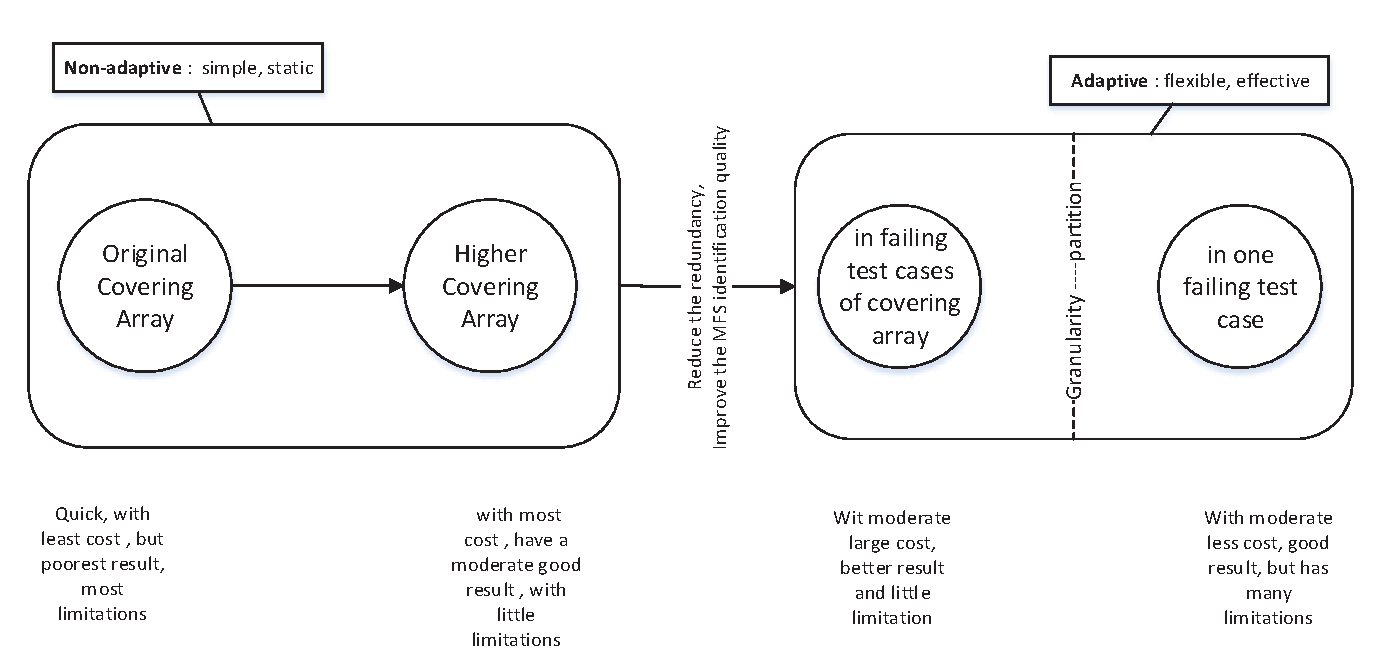
\includegraphics[width=5.6in]{MFSpartition.eps}
 \caption{A simple conclusion of the relationships between these MFS identification appraoches}
 \label{figch}
\end{figure*}


\section{Motivation of the approach}\label{sec:motiv}

Take OFOT for example, then illustrate the problems, and other similar approaches problems.

\subsection{Multiple MFS}
\subsubsection{Overlapping MFS}
\subsection{High degree MFS}
\subsection{Too many test cases}
\subsection{Needs too many computing resources}
\subsection{Introducing of newly MFS}

A big table that consists of many


\section{Theory foundation}\label{sec:propositinon}

\begin{assumption}

\end{assumption}




\begin{proposition}
All the schemas in a passed test configuration are healthy schemas.
All the subschemas of a healthy schemas are healthy schemas.
\end{proposition}
\begin{proposition}
If schema $s_{a}$ subsumes  schema $s_{b}$ ,schema  $s_{b}$ subsumes schema $s_{c}$, then $s_{a}$  subsumes $s_{c}$.
\end{proposition}
\begin{proposition}
All the parent-schemas of a faulty schema are faulty schemas.
\end{proposition}
\begin{proposition}
All the subschemas of a healthy schema are healthy schemas.
\end{proposition}

\subsection{weaken of the assumptions}

\section{The approach to identify the minimal failure-inducing schemas}\label{sec:app}
Based on these definitions and propositions, we will describe our approach to identify the failure-inducing schemas in the SUT. To give a better description, we will start give an approach with an assumption , and later we will weak the assumption.

\begin{definition}[candidate minimal faulty schema]
If a schema is a faulty schema and satisfy the followed condition:
1.none of its subschemas are faulty schemas, 2. at least one subschema is pending schema.(is need discuss!!!!!! one or none is okay?)We then call the schema a \emph{candidate minimal faulty schema}(\emph{CMINFS} for short).
\end{definition}
\begin{definition}[candidate maximum healthy schema]
If a schema is a healthy schema and and satisfy the followed condition:
1.none of its  parent-schemas are healthy schemas, 2. at least one subschema is pending schema. We then call the schema a \emph{candidate maximum healthy schema}(\emph{CMAXHS} for short).
\end{definition}



\subsection{additional failure-inducing not be introduced}
\begin{assumption}
Any newly generated test configuration will not introduce additional failure-inducing schemas.
\end{assumption}

There are similar assumptions defined in[][], however, it is a strong assumption, which we will change later. And still for this assumption, we can get the followed lemma which can help us to identify whether a pending schema is a healthy schema or a faulty schema.
\newtheorem{lemma}{Lemma}
\begin{lemma}
For a pending schema, we generate an extra test configuration that contains this schema. If the extra test configuration passes, then this schema is a healthy schema. If the extra test configuration fails, then the schema is a faulty schema.
\end{lemma}
\begin{proof}
According to definition of healthy schema, it is obvious that this schema is a healthy schema when the extra test configuration passes.

When the extra configuration fails, this is a faulty schema (or there exists no faulty schema and this test configuration would not fail because the assumption says that this newly generated configuration will not introduce additional faulty schemas).
\end{proof}

\subsection{framework to identify the minimal faulty schema}
As we can identify a pending schema to be healthy schema or faulty schema by generating newly test configurations, then the approach to identify the minimal faulty schema is clear. Fig.\ref{fig_overview} shows an overview of our approach. We next discuss each part of the approach in more detail.
\begin{figure}
 \centering
 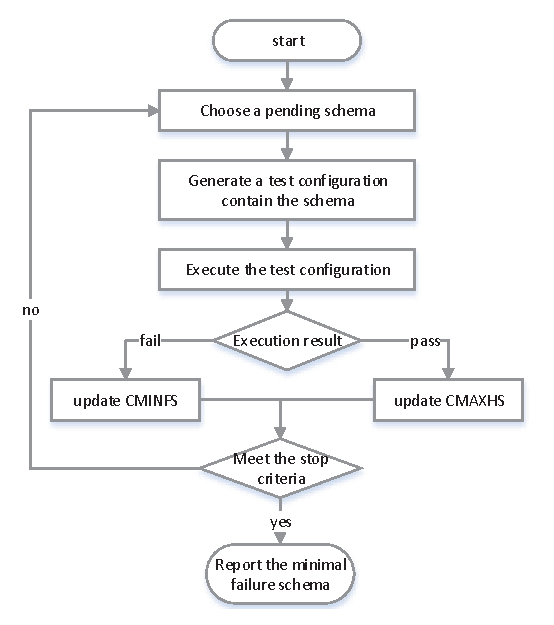
\includegraphics[width=2.7in]{gp.eps}
 \caption{Overview of approach of identifying MFS}
 \label{fig_overview}
\end{figure}
\subsubsection{Choosing a pending schema}
Before we think getting a pending schema, we should assume an general scenario. That is, we have already make sure some schemas to be healthy schemas and some schemas to be faulty schemas, then assume that we still don't meet the stopping criteria, we will choose a pending to check next. But first, we should make sure what schema is pending schema?

In effect, the schemas we can't make sure whether are faulty schemas nor healthy schemas are our wanted. Step further, we sperate this condition into two parts: 1. can't make sure it is faulty schema. As we already know some faulty schemas, then we just make the schema that first not be any one of these faulty schemas and not be the parent-schema of any one of these faulty schemas(As if not, it must be a faulty schema according to the proposition 3). 2 can't make sure it is healthy schema. Similar to the first condition,we already know some healthy schemas, then we just make the schema that first not be any one of these healthy schemas and not be the subschema of any one of these healthy schemas. It is obvious a pending schema must meet both the two conditions.

However, this is not the end of story of checking a pending schema. With the process of identifying, more and more faulty schemas and healthy schemas will be identified. It is not a small number, as it can reach to O($2^n$). So both for space and time restriction, we should not record all the faulty schemas and heathy schemas. Then we should find another way to check the pending schema.

To eliminate this problem, we propose an method which can check a pending schema with a small cost. It need to record the CMINFS and CMAXHS all through the process. Instead record all the faulty schemas and healthy schemas, CMINFS and CMAXHS are rare in amount, which can help to largely reduce the space need to record. Then according to the followed two propositions, we can easily check a pending schema.

\begin{proposition}
If a schema is neither one of nor the parent-schema of any one of the CMINFS, then we can't make sure whether it is a faulty schema.
\end{proposition}
\begin{proof}
Take a schema $s_a$, a CMINFS set $S_{cminfs}$ and a faulty schema $S_{fs}$ set which determined now. It is note that any element $fs_i \in S_{fs}$ must meet that either $fs_i \in S_{cminfs}$ or $fs_i$ be the parent-schema of one of the $S_{cminfs}$. Assume that $s_a$ is neither the one of nor the parent-schema of any one of the $S_{cminfs}$. To proof the proposition, we just need to proof that $s_a$ is neither the one of nor the parent-schema of any one of the $S_{fs}$.

As $s_a$ is neither the one of nor the parent-schema of any one of the $S_{cminfs}$, so it is not one of $S_{fs}$. Then we assume $s_a$ is the parent-schema of one of $S_{fs}$, say, $fs_j$. As $fs_j$ must meet either $fs_j \in S_{cminfs}$ or $fs_j$ be the parent-schema of one of the $S_{cminfs}$. So $s_a$ is the parent-schema of one of $S_{cminfs}$ according to the proposition 2, which is contradict. So the proposition is correct.
\end{proof}

\begin{proposition}
If a schema is neither one nor the the subschema of any one of the CMAXHS, then we can't make sure whether it is a healthy schema.
\end{proposition}
We ignore this proof as it is very similar to the previous one.

Up to now, we can judge whether a schema is a pending schema, but in effect, there are many pending schemas in a test configurations, especially at the beginning of our process. To choose which one has an impact on our approach. To better illustrate this problem, we consider the followed example:

Assume the failing test configuration: (1 2 1 1 1 2 1 2), that the CMINFS set: (1 2 1 1 - 2 - -) (- 2 - - 1 2 - 2), the CMAXHS set:(- 2 - - - - - -) (- - - - 1 - - -). We list some pending schemas followed (not all, as the number of all the pending schemas is too much that is not suitable to list here):

(1 2 1 - - 2 1 2) (- 2 1 1 - 2 - 2) (1 2 1 1 - - - -) (- 2 1 1 - 2 - -) (1 2 1 - - - - -) (- 2 - 1 - - 2 -) (1 2 - - - - - -) (- - 1 1 - - - -) (1 - - - - - - -)  (- - 1 - - - - -).

Choose what is really different. If we choose (1 2 1 - - - - -), assume we check it as a healthy schema. Then all its subschemas, such as (1 2 - - - - - -) (1 - - - - - - -)  (- - 1 - - - - -), are healthy schemas. It means that we did not need generate newly test configurations for them. But if we check it as a faulty schema, we can make sure all its parent-schemas are faulty schemas, in this case, they are (1 2 1 1 - - - -) and (1 2 1 - - 2 1 2) need no newly test configurations to test.

Let's look at this problem from another angle. Take the schema as a integer number, these parent-schemas of a schema is like the integer numbers bigger then this number, and these subschemas of a schemas is like the numbers smaller than this number. Take a float number as the metric, then, we can describe the faulty schema as the number bigger than this metric, and healthy schema as number smaller than this metric. So the minimal faulty schema is just the number most approximate the metric and bigger than the metric.

It seems like a search problem scenario. Then can we directly apply the efficiently algorithm binary-search? the answer is no, because there are schemas that neither parent-schema or subschema relationship, such as(1 2 1 - - 2 1 2) (- 2 1 1 - 2 - 2). So to utilize the binary search technique, we should make some change. First, should give the followed definitions:

\begin{definition}[chain]
A chain is an ordered sequences of schemas in which every schemas is the direct parent-schema of the schema that follows. Moreover,if all the schemas in a chain are pending schemas, we call the chain a pending chain.
\end{definition}
This definition is similar to the path in []

As all the schemas in a chain are have relationships, then we can apply binary search technique. As we all know, the longer the pending chain, the better performance binary search technique will get. So we should choose a pending chain as longer as possible each iteration.

To get a longest chain, we need to ensure that the head schema of this chain do not have any parent-schema which is a pending schema(called up pending schema), and the tail schema do not't have any subschema which is a pending schema (called down pending schema). The algorithm that get the up pending schemas and down pending schemas are list in algorithm 1 and algorithm 2.

As showed in algorithm 1, we start from the failing test configuration $\mathcal{T}$, assign it to the \emph{rootSchema}(line 1)and then add it to a \emph{lists}(line 3). We then do some operation (line 4 -line 12)to this lists and at last get these pending schemas in lists as up pending schemas.(line 13)  This operation consists of two iteration:

1. successively get one \emph{CMINFS} in $\mathcal{S_{CMINFS}}$. (line 4). Define a temple value \emph{nextLists} which initialize an empty set(line 5).We then execute the second iteration. After that, we will eliminate these same schemas list in \emph{nextLists} (line 10)and then assign to \emph{lists} (line 11).

2. Successively get one schema in \emph{lists}(line 6). And then mutant it according to the \emph{CMINFS} to a set of schemas(line 7). Add them to the  \emph{nextLists} (line 8).

The mutant procedure for a schema is just remove one value in it which this value is also in \emph{CMINFS}. This procedure will result in \emph{k} mutant schemas if the \emph{CMINFS} is a \emph{k}-value schema. By doing this, any mutant schema will not be the parent-schema of the corresponding \emph{CMINFS}.

After this two iteration, the schemas in the \emph{lists} will not be the parent-schema of any \emph{CMINFS} in the $\mathcal{S_{CMINFS}}$.

\begin{algorithm}
  \caption{getting up pending schema}
  \begin{algorithmic}[1]
     \Require  $\mathcal{T}$ \Comment{failing test configuration}

     $\mathcal{S_{CMINFS}}$ \Comment{set of CMINFS}

     $\mathcal{S_{CMAXHS}}$ \Comment{set of CMAXHS}

     \Ensure  $\mathcal{S_{UPS}}$ \Comment{the set of up pending schemas}

    \Statex\Comment{\%comment: initialize\%}
    \State $rootSchema \leftarrow \mathcal{T}$
    \State $lists \leftarrow \emptyset$
    \State $lists \cup \{rootSchema\}$

    \ForAll{$CMINFS$ in $\mathcal{S_{CMINFS}}$}
     \State $nextLists \leftarrow \emptyset$
     \ForAll{$schema$ in $lists$}
        \State$S_{candidate} \leftarrow mutant_{r}(schema,CMINFS)$
        \State $nextLists \leftarrow nextLists \cup S_{candidate}$
     \EndFor
     \State $compress(nextLists)$
     \State $lists \leftarrow nextLists$
    \EndFor
     \State $\mathcal{S_{UPS}} \leftarrow   \{ s | s \in lists \wedge {s\ is\ pending}\}$
  \end{algorithmic}
\end{algorithm}

Fig.\ref{figch} gives an example to the algorithm 1.

\begin{figure}
 \centering
 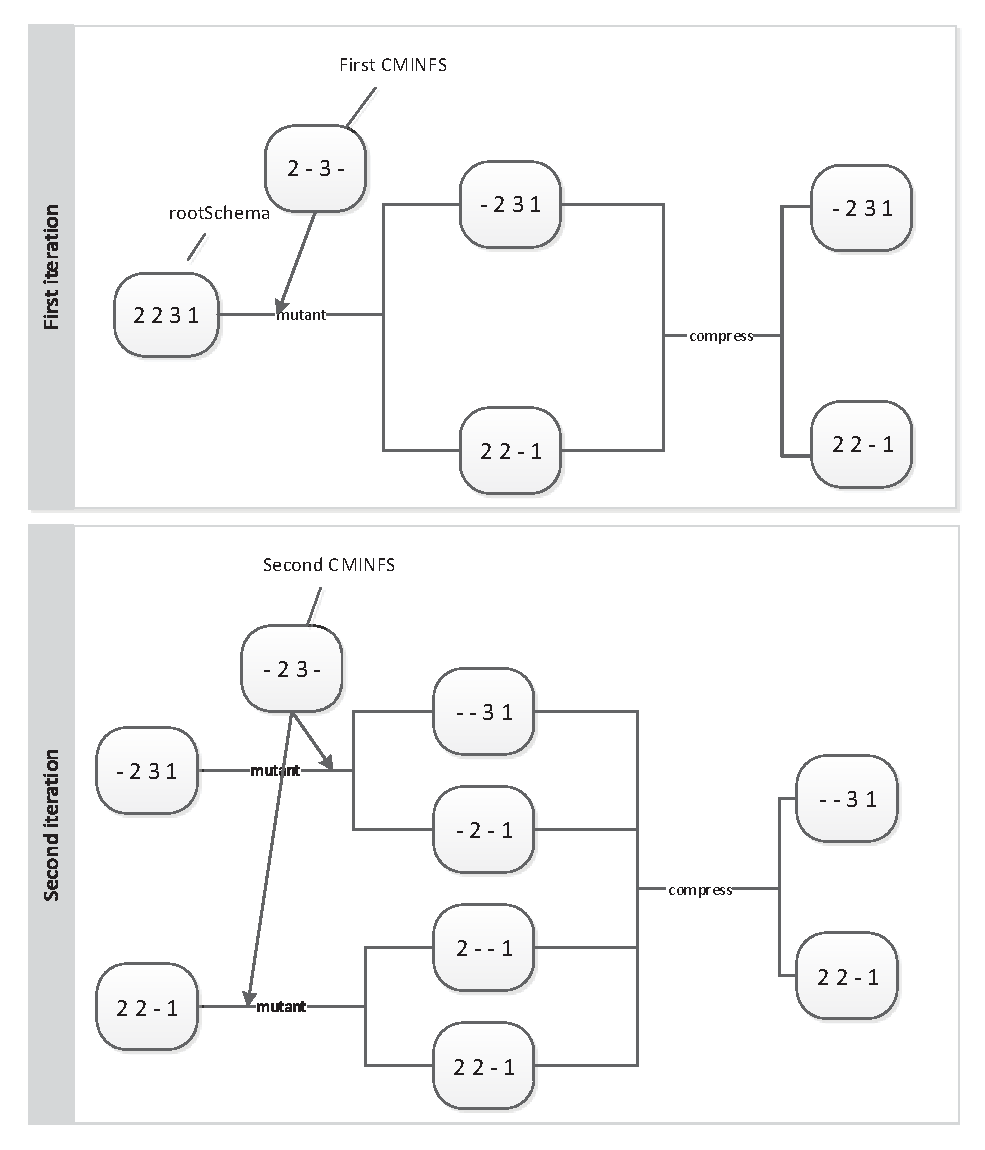
\includegraphics[width=2.8in]{ch.eps}
 \caption{example of getting up pending schemas}
 \label{figch}
\end{figure}


Algorithm 2 is a bit different from algorithm 1. As our target is to get the minimal value pending schema, we get started from a 0-value schema(line 1). Then to make schemas not to be the subschema of any \emph{CMAXHS} in $\mathcal{S_{CMAXHS}}$, we should let the schemas must contain at least one value that is not in the corresponding \emph{CMAXHS}. So the strategy is to get a reverse schema of the \emph{CMAXHS} which this schema consists of all these values in the failed configuration except these are in \emph{CMAXHS}(line 5). And mutant the schema by adding one value in the reversed schema to make the schma not to be the subschema of the correspinding \emph{CMAXHS}(line 8). After two iteration similar to Algorithm 1, we will get all the schemas that meet that not to be  subschema of any \emph{CMAXHS} in $\mathcal{S_{CMAXHS}}$ from which we choose these pending schemas as down pending schemas(line 14).


\begin{algorithm}
  \caption{getting down pending schema}
  \begin{algorithmic}[1]
     \Require  $\mathcal{T}$ \Comment{failing test configuration}

     $\mathcal{S_{CMINFS}}$ \Comment{set of CMINFS}

     $\mathcal{S_{CMAXHS}}$ \Comment{set of CMAXHS}

     \Ensure  $\mathcal{S_{DOWNS}}$ \Comment{the set of down pending schemas}

    \Statex\Comment{\%comment: initialize\%}
    \State $initschema \leftarrow \mathcal{()}$
    \State $lists \leftarrow \emptyset$
    \State $lists \cup \{initschema\}$

    \ForAll{$CMAXHS$ in $\mathcal{S_{CMAXHS}}$}
     \State $reverse \leftarrow \ reverse(CMAXHS)$
     \State $nextLists \leftarrow \emptyset$
     \ForAll{$schema$ in $lists$}
        \State$S_{candidate} \leftarrow mutant_{a}(schema,reverse)$
        \State $nextLists \leftarrow nextLists \cup S_{candidate}$
     \EndFor
     \State $compress(nextLists)$
      \State $lists \leftarrow nextLists$
    \EndFor
     \State $\mathcal{S_{DOWNS}} \leftarrow   \{ s | s \in lists \wedge {s\ is\ pending}\}$
  \end{algorithmic}
\end{algorithm}

Fig.\ref{figct} gives an example to the algorithm 2. we can see.
\begin{figure}
 \centering
 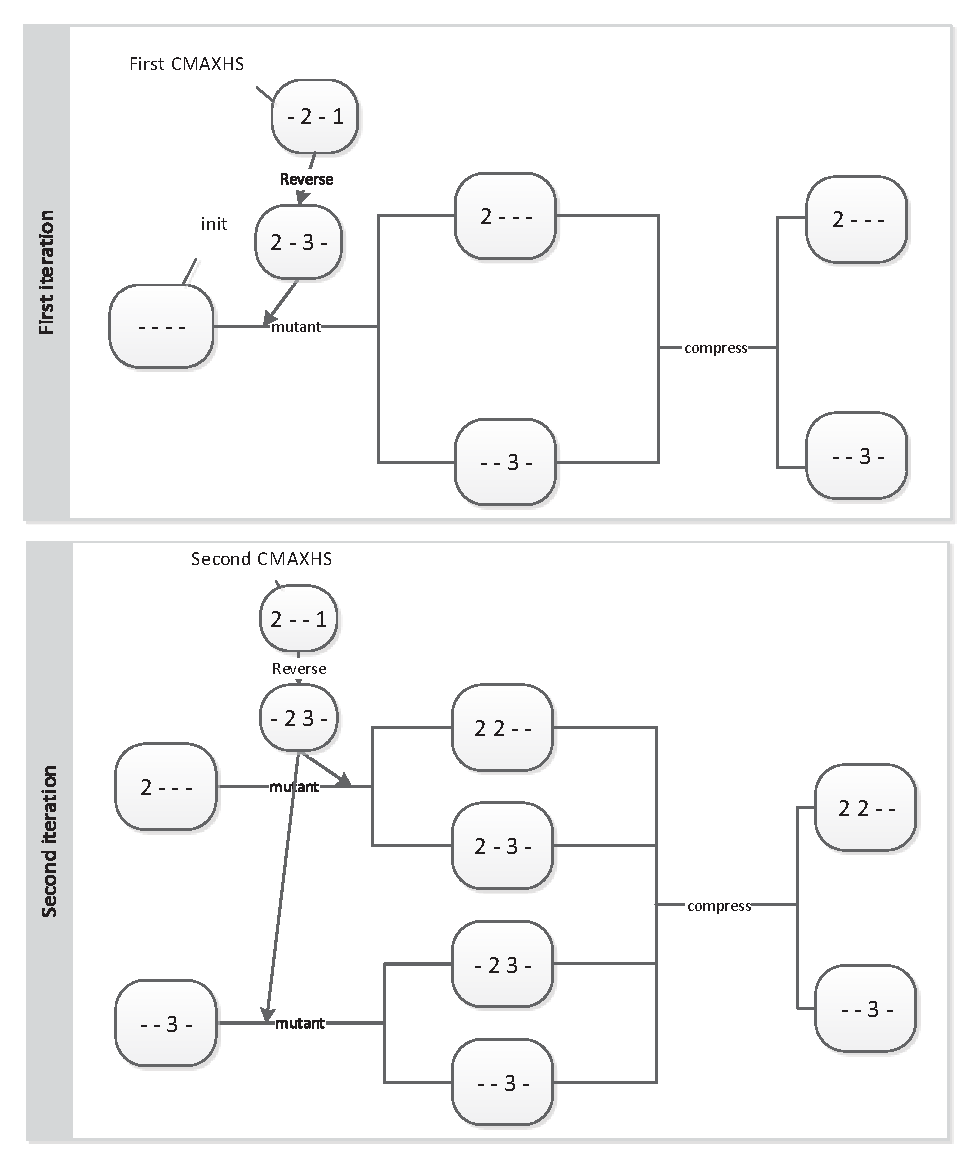
\includegraphics[width=2.8in]{ct.eps}
 \caption{example of getting down pending schemas}
 \label{figct}
\end{figure}

After we can get the up pending schemas and down pending schemas, then the algorithm of getting the longest chain can be very simple,which is list in Algorithm 3. In this algorithm we can see that we just search through the up pending schemas and down pending schemas(line 7 - 8) to find the two schemas which has the maximum distance(line 9 - 13). The distance of a k-value schema and a l-value schema (k>l) is defined as:

$$distance(S_k, S_l) =
\begin{cases}
-1, & S_k\ is\ not\ parent-schema\ of\ S_l\\
k-l,& otherwise
\end{cases}
$$

Then we just use \emph{makechain} procedure to generate the longest chain. The \emph{makechain} procedure is very simple, it just repeat adding one schema by keeping all the value in down pending schema and removing one factor of the previous schema.

\begin{algorithm}
  \caption{Finding the longest pending schema}
  \begin{algorithmic}[1]
     \Require  $\mathcal{T}$ \Comment{failing test configuration}

     $\mathcal{S_{CMINFS}}$ \Comment{set of CMINFS}

     $\mathcal{S_{CMAXHS}}$ \Comment{set of CMAXHS}

     \Ensure  $\mathcal{CHAIN}$ \Comment{the chain}
    \State $\mathcal{S_{UPS}} \leftarrow getUPS(\mathcal{T},\mathcal{S_{CMINFS}},\mathcal{S_{CMAXHS}}) $
    \State $\mathcal{S_{DOWNS}} \leftarrow getDOWNS(\mathcal{T},\mathcal{S_{CMINFS}},\mathcal{S_{CMAXHS}}) $
    \State $max \leftarrow 0$
    \State $head \leftarrow NULL $
    \State $tail \leftarrow NULL $
    \State $chain \leftarrow NULL $
     \ForAll{$up$ in $S_{UPS}$ }
        \ForAll{$down$ in $S_{DOWNS}$}
            \If {$distance(up, down) \geq max$}
              \State $max \leftarrow distance(up, down)$
              \State $head \leftarrow up$
              \State $tail \leftarrow down$
             \EndIf
        \EndFor
     \EndFor
     \State $\mathcal{CHAIN} \leftarrow  makechain(head, tail)$
  \end{algorithmic}
\end{algorithm}

The last step of getting the schema is just choose the schema from the longest chain. To clearly describe the approach, we discuss it in the overall identifying algorithm which is list in the Algorithm 4. As we have talked previously, we first judge the end criteria, if meet we will report the minimal faulty result. Otherwise we will do the loops. In the loop, we first judge if it is the beginning or headIndex greater than tailIndx, then we will update the CMINFS and CMAXHS, followed generated the longest chain and initial the headIndex, tailIndex and middleIndx. If not we will get the middleIndex indicate the half. Then will select the schema with index of middleindex in the longest chain. And then generate a test configration and exectute the SUT under it. If the result passed, we let tail = middle - 1 else head = middle + 1. By doing this and the previous set the middleIndex we can apply the binary searh to the indentying. It is noted that we intitally let middle = 0. which we want know if this chain has faulty schema as soon as possible.
\begin{algorithm}
  \caption{identify process}
  \begin{algorithmic}[1]
    \Require  $\mathcal{T}$ \Comment{failing test configuration}

     $\mathcal{S_{CMINFS}}$ \Comment{set of CMINFS}

     $\mathcal{S_{CMAXHS}}$ \Comment{set of CMAXHS}

     \While{$hasn't\ meet\ the\ end\ criteria$}
       \If{$the\ beginning$ or $headIndex > tailIndex$}
       \State $update(\mathcal{S_{CMINFS}},\mathcal{S_{CMAXHS}})$
       \State $longeset \leftarrow getLongest( \mathcal{T},\mathcal{S_{CMINFS}},\mathcal{S_{CMAXHS}})$
       \State $headIndex \leftarrow 0$
       \State $tailIndex \leftarrow length(longest) - 1$
       \State $middleIndex \leftarrow 0$
     \Else
       \State $middleIndex \leftarrow \frac{1}{2} \times (tailIndex + headIndex)$
     \EndIf
       \State $\mathcal{SCHEMA} \leftarrow longest[middleIndex]$
       \State $generate\ a\ extra\ test\ configration\ \mathcal{T'}\ contain\ \mathcal{SCHEMA}$
       \State $execute\ SUT\ under\ \mathcal{T'}$
     \If{$the\ test\ configration\ passed$}
       \State $tailIndex \leftarrow middleIndex - 1$
     \Else
       \State $headIndex \leftarrow middleIndex + 1$
     \EndIf
   \EndWhile
   \State $report\ the\ minimal\ faulty\ schemas$
  \end{algorithmic}
\end{algorithm}

\subsubsection{generate a new test configuration}
To generate a new test configuration to test the schema. The generated test configuration must meet the followed rules:

1. must contain the selected schema.

2. must not

3. constraint(system-wide constraint and test case specific constraint, i.e., masking effect)

The first one is easy to meet. We just keep the same value which are in the schema are also in the test configuration.
We must meet the second condition for that if we contain another one, combine this then this test configuration will contain an parent-schema of this selected schema in the original test configuration, and it will confuse us whether it is indicate this schema or its parent-schemas dedicate this result. To fulfil this condition, we need to choose other available values in the SUT which are different from the original test configuration.
the third one is that we should consider the constraints

\subsubsection{execute SUT under the test configuration}
In real software testing scenario, when we test a SUT under a test configuration, there may be many possible testing state: such as pass the testing assertion, don't pass the testing the assertion but with different failure type, can't complete the testing. To get a clear discussion, in this paper we just use \emph{pass} represent the state that pass the testing assertion and \emph{fail} represent all the remained state.

\subsubsection{update information}
The update information is followed when the current chain is checked over. Then before we generate another longest chain, we should update the CMINFS and CMAXHS set. In fact, we just need the CMINFS and CMAXHS in the longest chain.

\subsubsection{stop criteria}
The stop criteria is clear, our algorithm stops when there are no pending schemas left, for that when we once can checked all the schemas of a test configuration, we can get the minimal faulty schemas, which is the target of our algorithm. And whether there are pending schemas can be easily checked by that if we can't generate a longest chain (the length must greater than 1), there must be no pending schemas.
\subsubsection{report the reuslt}
In fact, the last in the CMINFS lists is must be the minimal faulty schemas. For that if these schema in the CMINFS is not minimal faulty schema, then there must be some pending schemas. However, the algorithm stop when there are no pending schemas remained. So at last these in the CMINFS must be the minimal faulty schemas.

\subsubsection{new ideas}
you should first identify a failure-inducing schema, and then find others. initial the find tuples, and then using the same algorithms as others. when identify is confirm ,  then choosing new longest path.

\subsection{example}
We will give an complete example listed in Table \ref{identifying_example}. Assume that a SUT is . constaints.
\begin{table*}\renewcommand{\arraystretch}{1.3}
  \caption{An example of identifying} \centering
  \label{identifying_example}
  \begin{tabular}{c|c|c|c|c|c}\hline
  \hline
  \bfseries $\mathcal{S_{CMINFS}}$ &   \bfseries $\mathcal{S_{CMAXHS}}$ & \bfseries Longest Chain & \bfseries Choosing Schema & \bfseries Generating Test Configuration & \bfseries Execution result\\
  \hline
  1 & 1 & 1 & 1 & 1 & false \\
   1 & 1 & 1 & 1 & 1 & pass\\
  1 & 1 & 1 & 1 & 1 & false\\
  \hline
  \end{tabular}

\end{table*}

\subsection{Without Safe Values Assumption}
Up to now our algorithm is based on the assumption that additional generated test configuration does not introduce newly faulty schema. We will give an augment algorithm this section to eliminate this assumption.
Our augment algorithm is inspired by the feedback machinery in the controlling system, which in high level we will validate the identify result at the end of the aforementioned algorithm, and if the schema is validated as a minimal faulty schema, we will end the algorithm, otherwise we will repeat the algorithm again to adjust the result. The detail of our augment algorithm is list in Algorithm 5. We can find the first part of augment algorithm is an unlimited loop, in the loop we first use previous identify algorithm to identify the MFS, and then we will check the result, the check process is just to addtional generate another test configurations and execute. When we find the MFS is not right, which means our process introduce newly MFS, then we first label this MFS as an healthy schema, and then update the CMAXHS. After check, if we find at least one MFS is not right, we then empty the CMINFS, and then readd these right identified MFS to this set, and then reprocess this process untill all the MFS is validated as right. The second part of our algorithm is just we look through the generated test cases one by one, if it failed, and did not contain the MFS we identified in the first part, which means it introduce newly faulty schema, and we will rerun this process to find these introduced MFS.
\begin{algorithm}
  \caption{augment identify process}
  \begin{algorithmic}[1]
    \Require  $\mathcal{T}$ \Comment{failing test configuration}

     $\mathcal{S_{CMINFS}}$ \Comment{set of CMINFS}

     $\mathcal{S_{CMAXHS}}$ \Comment{set of CMAXHS}

     \While{$true$}
       \State $\mathcal{S_{MFS}} = Identify\_process(\mathcal{T})$
       \ForAll{$MFS$ in $\mathcal{S_{MFS}}$}
       \If{$validate(MFS) = fail$}
         \State $updateHealthySchemas(S_{CMAXHS},MFS)$
       \EndIf
       \EndFor
       \If{$at\ least\ one\ MFS\ is\ not\ correct$}
          \State $empty(S_{CMINFS})$
          \State $add\ all\ the\ vaildated\ MFS\ in\ the \mathcal{S_{CMINFS}}$
       \Else
           \State $break$
       \EndIf
      \EndWhile
      \ForAll{$testCase$ in $\mathcal{EXTRATESTCASES}$}
         \If{$testCase\ introduce\ newly\ MFS$}
           \State $augment\_identify\_process(testCase)$
         \EndIf
      \EndFor
      \State $report\ the\ minimal\ faulty\ schemas$
  \end{algorithmic}
\end{algorithm}

Table \ref{augment_example} illustrate this augment algorithm with an example.
\begin{table*}\renewcommand{\arraystretch}{1.3}
  \caption{An example of augment identifying} \centering
  \label{augment_example}
  \begin{tabular}{c|c|c|c|c|c}\hline
  \hline
  \bfseries $\mathcal{S_{CMINFS}}$ &   \bfseries $\mathcal{S_{CMAXHS}}$ & \bfseries Longest Chain & \bfseries Choosing Schema & \bfseries Generating Test Configuration & \bfseries Execution result\\
  \hline
  1 & 1 & 1 & 1 & 1 & false \\
   1 & 1 & 1 & 1 & 1 & pass\\
  1 & 1 & 1 & 1 & 1 & false\\
  \hline
  \end{tabular}

\end{table*}

\section{Evaluation with simulated SUT} \label{sec:simulateEx}
In this section, we designed a simulated SUT of which the number of parameters and the value of each parameter can both be customized. In addition, we can also manually inject faulty schemas in the simulated SUT. We will conduct a series of experiments with this simulated SUT in this section. The goal of our experiments is to evaluate the efficiency and effectiveness of our approach compared with other existed techniques. The main reason why we use simulated program is that we can easily run a bench of experiments with various states of a SUT, i.e., different parameters and different MFSs. By doing so we can thoroughly learn the performance of each algorithm without biases.

As we discussed in the background section, the fault privilege properties just effect the way we determine a configuration is fail or pass. It doesn't effect the performance of each algorithm. So to be simple and clear, we omit the fault privilege in the simulated SUT , i.e., all the fault in the SUT has the same privilege. This is a ideal scenario which may not exist in real softwares, in the empirical studies of section 7 we will deal with the real faults in some open-source softwares with different privileges.
\subsection{comparison algorithms}
There are several algorithms aim to identify the MFS, they can be classified as non-adaptive methods and adaptive methods. The first set of methods do not need additional test configurations and can identify the MFSs when given an executed test configurations while the second one will generate some more additional test configurations to facilitate the process of identifying MFSs in a failing test configuration. Our algorithm is belong to the second part. To make the comparison clear and fair, we just choose the algorithms which all belong to the second part as the comparison subject, i.e., adaptive methods. These algorithms is listed as follows:

(1)OFOT, proposed by Nie[], it change one factor of a test configuration one time to generate a newly configuration and then analysis the MFSs according to the executed result of these generated configurations. (2)FIC-BS, proposed by Zhang, using a delta debugging strategy to isolate the MFSs (3) LG, proposed by Martine[], use a locatable graph to represent the faulty schema and adopt divide and conquer strategy to find the MFSs. (4) SP[], proposed by Ghandehari, they generate configurations for these mostly suspicious schemas and give a rank of these schemas at last based on the suspicious "degree" of them (5) CTA, proposed by Shakya[], it combine the OFOT strategy and the classified tree technique which first applied in characterize the MFS in [] to analysis the MFSs. (6)RI, proposed by Li[], it is also using delta debugging, but the factors needed to change in a iteration are different from FIC-BS at some conditions.(7)IterAIFL, proposed by Wang[], a mutant based on OFOT, which changes different number of factors instead of one each iteration for a test configuration. (8)TRT and TRT-NA, two approaches proposed in our previous work[], using a structured tree model to analysis the MFSs in a failing configurations.  More details of these algorithms will be discussed in the related works.

Some parameters of these algorithm are assigned: for SP, the degree of MFSs we set is 2(except for the last group of experiment, which is 4 instead), for CTA,the confidence factor of classified tree algorithm is 0.25 as same as [].
\subsection{evaluation metrics}
There are three facts we care about each algorithm: 1)How many additional test configurations do an approach need to generate? 2)How many MFSs can an approach identify for a SUT? 3)Does all the schema identified by an approach are correctly? We will define two formula to represent the second and third facts respectively, i.e., recall and precise:
$$recall =
 \frac{correctly\ Identiied\ MFS}{all\ the\ MFS\ in\ SUT}
$$

$$precise =
 \frac{correctly\ Identified\ MFS}{all\ the\ identified\ MFS}
$$
The recall is percentage of the correctly identified MFSs of an algorithm of all the MFSs in the SUT. The bigger the metric the better an approach can perform on finding MFSs in a SUT. There are some factors may influence this metric of an algorithm, mainly are whether an approach consider a failing configurations contain multiple MFSs, whether consider if there exist overlapped MFSs in a failing configurations and whether consider the newly introduced MFSs of the additional generate configurations.  The precise is the percentage of the number of correctly identified MFSs of algorithm of all the number of  MFSs this algorithm identified. This metric measure the accurately of an approach and the bigger it is the better the approach performs. This metric is related to whether a algorithm consider the influence if an generated test configuration contain newly MFSs. If the approach did not consider so, it may make a wrong judgement to determine some schemas in the original configuration to be faulty schemas which in fact are not.

Of course these factors we mentioned are just affect these the no-machine learning algorithm, as for the machine learning algorithms,i.e., CTA, the factor that matters is the classified algorithms itself.


\subsection{experiment setups}
We will carry out the followed five experiment in this section:

1)For the first one, we will give a set of SUTs with 8 parameters, each parameter has 3 values, all of them only have one MFS, the difference between each SUT in this set is the MFS we inject in it. All the MFSs has the degree of 2. There are $\binom{8}{2} = 28$ possible MFSs we can inject, so the number of set of SUTs is 28. For each SUT in this set, we will feed each algorithm the same failing configurations contain the MFS we inject, and then let these algorithm identify the MFS in it. We will record the additional configurations each algorithm needed. As the first experiment is simple, so all the approaches can identify the MFS with precise 1 and recall 1. This experiment will give us a initial view of the cost of each algorithm on identifying the MFS in a failing configuration.

2)The second experiment is similar to the first one, except that we will inject double different MFSs with degree 2 in each SUT. It is easily compute their are  $\binom{28}{2} = 278$  possible SUTs in this experiment. For each algorithm, we also feed them with the same failing configuration contain the two MFSs and then let them identify them. Another difference from the experiment 1 is that in this experiment we will record the "recall" and "precise" of each algorithm, as these metric is not equal to 1 for all the algorithms like experiment 1. This experiment mainly focus on observing the performance of each algorithms in facing multiple MFSs in a configuration.

3)The third experiment aims at learning the capability that each algorithm handling the introducing newly MFSs. To accomplish this goal, We firstly inject two MFSs in a SUT, and then feed each algorithm a failing configuration which contain only one MFS,  remaining another MFS not in it. To increase the possibility of introducing newly MFSs for each algorithm, we set the second MFS with degree 1, which may be easily introduced by just changing one factor of the original failing configuration.  The first MFS in the original configuration has degree 2. So there are  $\binom{8}{2} \times \binom{8}{1} = 224$ possible SUTs in this experiment. The same as experiment 2, we will record the "recall" and "precise" of each algorithm.

4)For the fourth experiment, we will vary the number of parameters of SUT. In specific we will take 8, 9, 10, 12, 15, 20, 30, 40, 60, 80, 100, 120 respectively as the number of parameters of SUT. For each number of parameters, say n, we will generate $\binom{n}{2}$ SUTs with different MFSs injected. And for these SUT, we will do the same process as experiment 1. At last we will record the average number of additional configurations each algorithm needed for each number of parameters. The goral of this experiment is to see the influence of the number of parameters on each approach.

5)In the fifth experiment we will fix the number of parameters of SUT to be 8, but vary the number of degrees of the MFS we inject in the SUT. That is, we will inject MFS in SUT with degrees 1,2,3,4,5,6,7,8 respectively, for a degree of m (m = 1,2,3,4,5,6,7,8), we will generate $\binom{8}{m}$ SUTs with different m-degree MFS injected. And then we will do the same thing as experiment 4 , i.e., record the average number of additional configurations each algorithm needed for each number of degree. This experiment is order to inspect whether these algorithm can handle different degree of MFS in a failing configuration.

\subsection{results and discuss}
We will discuss the results into five groups according to the experiment set up.

1)The result of the experiment 1 is depicted in figure \ref{fig_single}. The y-axis report the number of configurations and the x-axis represent a SUT. Algorithms differs from each other in the signal of point and the line linking these points. For a particular algorithm, a point indicate the number of configurations corresponding to the y-axis needed for identifying the MFS in the SUT which corresponding to the x-axis of this point.

There are some intuitive information we can learn from this figure. First, the configurations needed of some algorithms didn't change along with the change of SUT. These algorithms are AIFL, CTA, OFOT,LG, while others need different configurations according to the SUT they are facing. Second, some algorithms(sp, aifl, trtNA, OFOT, CTA) shows a obvious disparity in this figure, we can easily rank them according to the number of configurations, i.e., $ofot = cta < trtNA < sp< aifl $. Besides, These algorithms needs more configurations than the remaining algorithms.

For the remaining algorithms, their results are tangled with each other. So in order to rank them, we give an average configurations each algorithms needed : Chain 9.25, FeedBack 11.25, fic 7.96, ri 8 ofot 16 lg 11 , sp .29, aifl 36, trt 10.75 trt-NA 23.75   CTA 16. Overall, we can conclude an initial rank in the number of configurations each algorithm needed as:  $FIC-BS<RI<LG<TRT<CHAIN<OFOT = CTA <TRT-NA<AIFL<SP$.

\begin{figure}
 \centering
 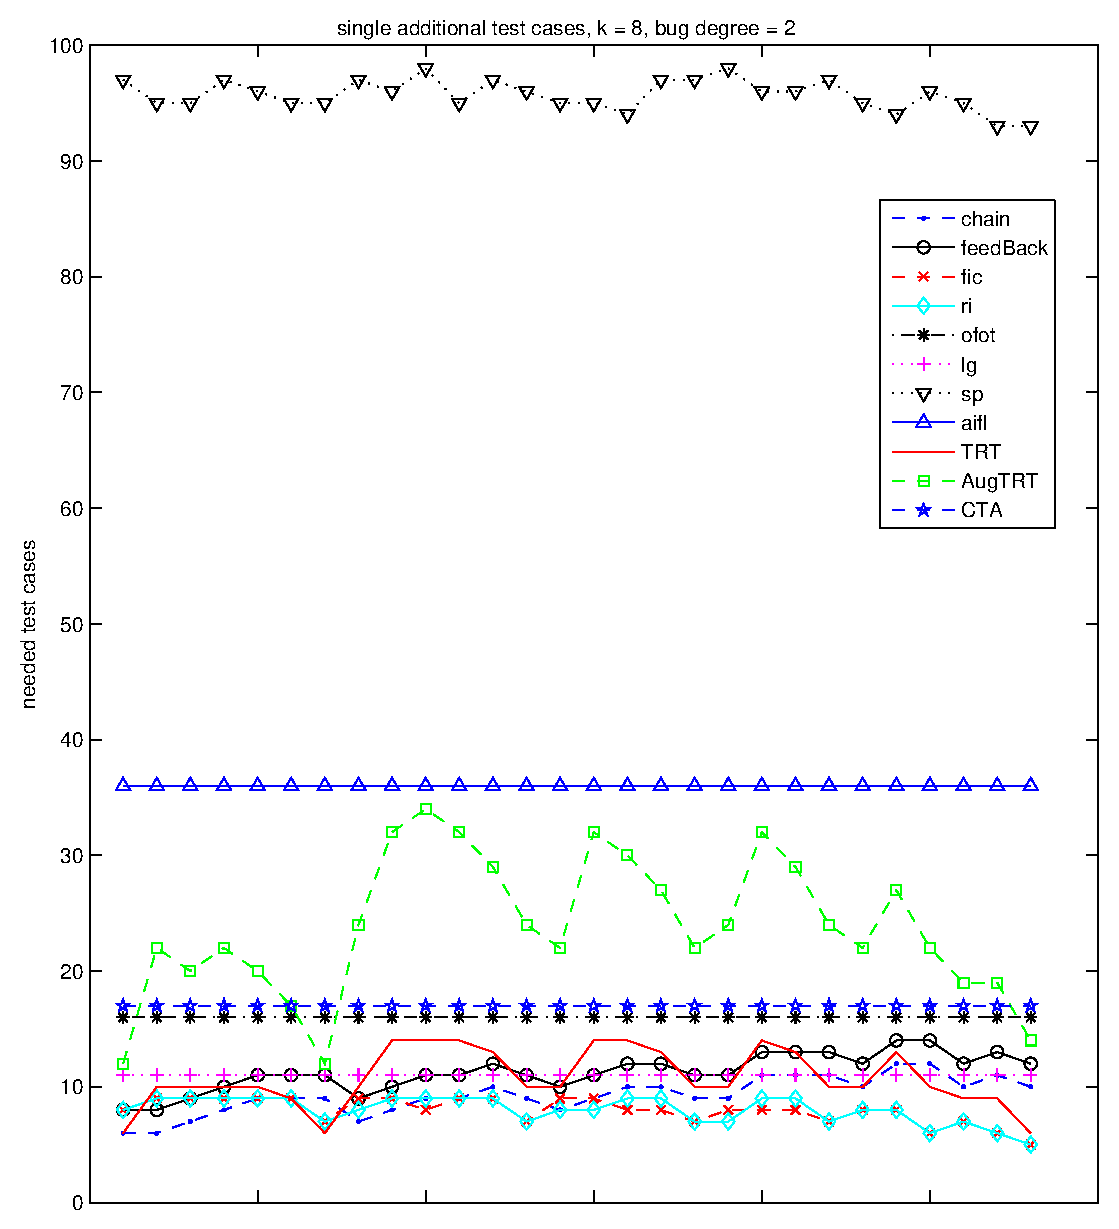
\includegraphics[width=2.8in]{single.eps}
 \caption{k = 8, t = 2,single, additional test suites}
 \label{fig_single}
\end{figure}

2)Figure \ref{fig_double} list the result of experiment 2. This figure doesn't show the number of configurations of each algorithms,instead it just show the average precise and recall for each algorithms as not all these algorithms can both get recall 1 and precise 1 as experiment 1. It is obvious meaningless if we compare two algorithms that one algorithm can reach recall 1 and precise 1 while the other can't. So we will only list the average number configurations of these algorithms that can reach recall 1 and precise 1 later.

From this figure, we can find the following algorithms: chain, lg, sp, aifl, trt and trt-na can both get the precise and recall 1, which means that they can perfectly deal with the multiple MFSs in a failing configuration. As the opposite side, algorithms OFOT and CTA both get the recall 0 and precise 0. This is a signal that the two algorithms can't handle the condition that a failing configuration contain multiple MFSs. So for these two algorithms, they may need other techniques to assist them in facing such conditions.  As for the remaining algorithms RI and FIC, they got precise 1 , but didn't reach recall 1, this is because they can't handle the condition if two MFSs have overlapped part. When they facing such condition, they can only identify one MFS of them.

The average number of configurations of these algorithms can both get recall and precise 1 is as follows:

we can find that our approach can also get a no-bad result among them

\begin{figure}
 \centering
 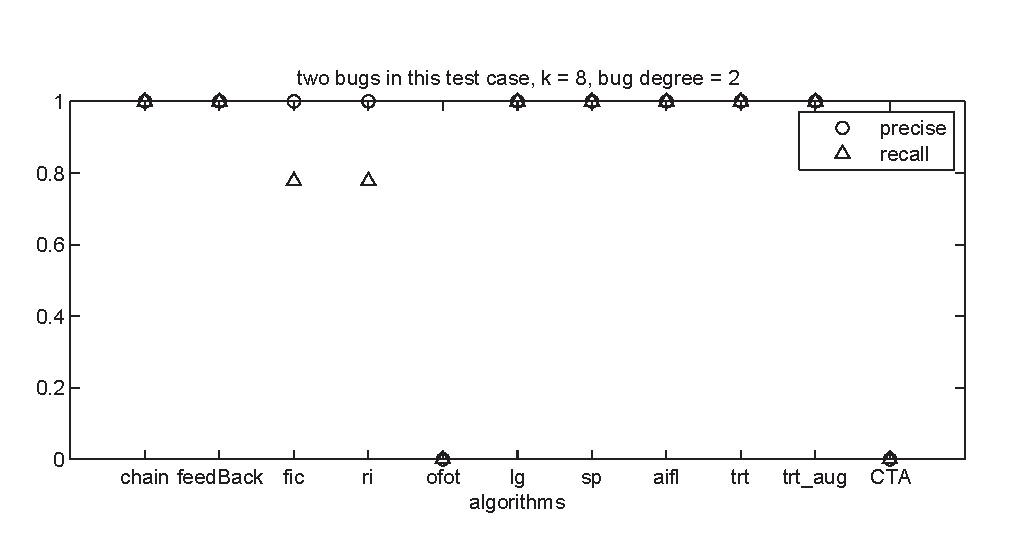
\includegraphics[width=2.8in]{d-8-2.eps}
 \caption{k = 8, t = 2,double, additional test suites}
 \label{fig_double}
\end{figure}

3)The third experiment's result is shown in fig \ref{fig_import}. Similar to experiment 2, this figure just record the recall and precise of each algorithm. We can learn several facts of this result.

First, no algorithm can both get recall 1 and precise 1 in this condition. Thus shows that no algorithm can perfectly handle the importing problem.

Second, even though, there are some algorithm(OFOT, LG, SP, TRT-NA, our approach is almost get precise 1) can get precise 1, this is a signal that the importing problem has a little impact on them

Third, our approach get the highest score in recall than others, the specific rank are $Chain > OFOT > LG = SP = TRT-NA > CTA > AIFL > TRT > FIC = RI$. It shows that our approach can find more MFSs than others when just feeding a failing configuration.

Fourth, algorithms fic and ri really suffers from this condition, as they get both recall and precise 0.

\begin{figure}
 \centering
 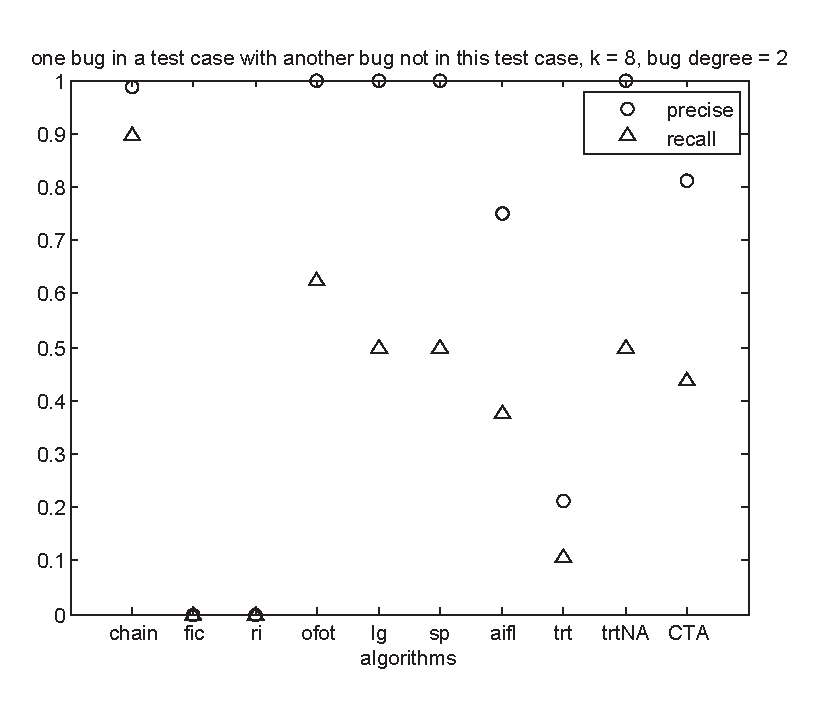
\includegraphics[width=2.8in]{i-8-2.eps}
 \caption{k = 8, t = 2,import, additional test suites}
 \label{fig_import}
\end{figure}

4)The data depicted in figure \ref{fig_free_k} shows that the average configurations needed of each algorithm for experiment 4. In this figure, the y-axis still reports the number of configurations while the x-axis represent a set of SUTs with the same number of configurations. These number of parameters are 8, 9, 10, 12, 15, 20, 30, 40, 60, 80, 100 and 120 respectively. And a point in this figure indicate the average number of configurations needed for the corresponding algorithm to identifying the MFS in these SUT with the same number of the parameters. For example, for the point whose x-axis is 8 corresponding to the algorithm "AIFL", we record the number of configurations needed to identify each SUT from the SUT with 8 parameters (totally $\binom{8}{2} = 28$ SUTs) and compute the average value of them, i.e., "".

We can easily learn that AIFL needs the largest number of configurations to identify MFS. Worse more, it need such big computing resource along with increase of k so that we even can't make it to identify the MFS in the SUT with number of parameters bigger than 12.  The second largest is the algorithm "SP". Although it needs much smaller computing resource than "AIFL", we yet can't tolerate the time it need to identify the MFS with number of parameter bigger than 40.

\begin{figure}
 \centering
 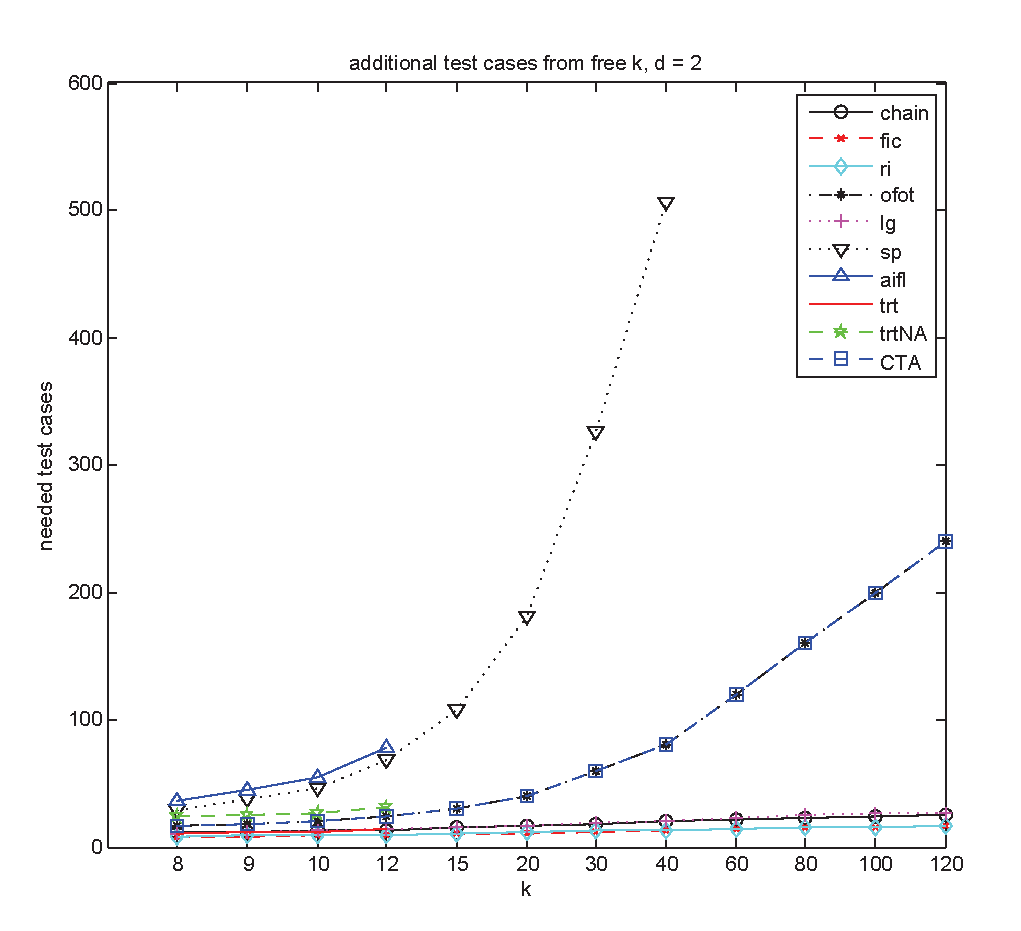
\includegraphics[width=2.8in]{k-2-s.eps}
 \caption{k is free, t = 2,single, additional test suites}
 \label{fig_free_k}
\end{figure}

As the average number of configurations of "SP" increase quickly with the increase of k. It make the results of the remaining algorithms show unclearly in this figure. To get a better view of the remaining algorithms, we enlarge the  perspective for these algorithms in figure \ref{fig_free_k_small}.

From this perspective, we first find that our previous approach TRT and TRT-NA also suffer from the large k. We can't let them identify the MFS with k bigger than 12. Apart form this two algorithms, all the remaining algorithms: chain, fic, lg, ri can complete this experiment. second, it also give us a intuitive rank of each algorithms according to the cost of configurations generated, i.e., $TRT-NA > LG > CHAIN > TRT > RI > FIC$. Combine With the two algorithms "AIFL" and "SP" we mentioned before, the final rank is $AIFL > SP > TRT-NA > LG > CHAIN > TRT > RI > FIC$.

\begin{figure}
 \centering
 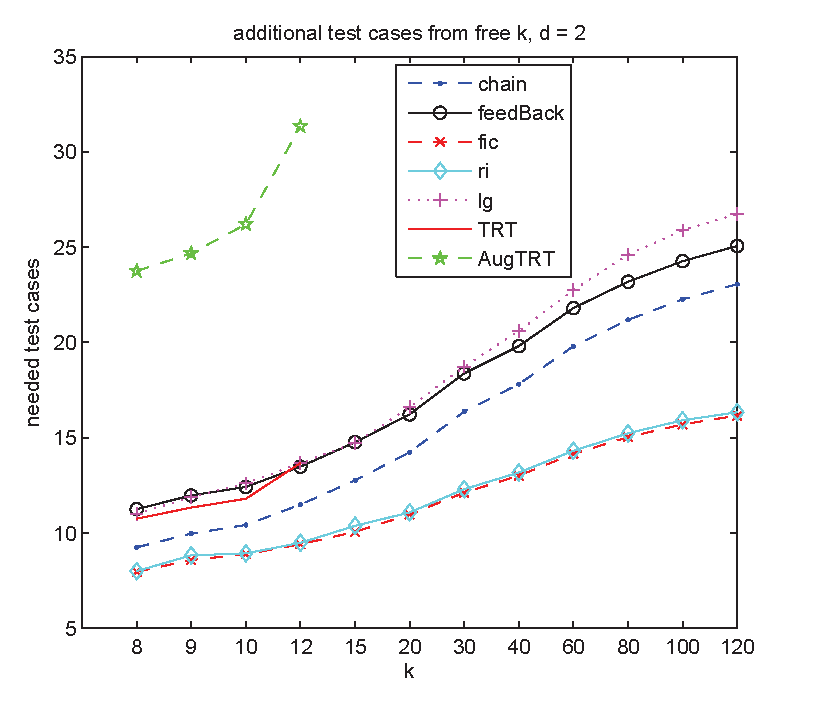
\includegraphics[width=2.8in]{k-2-s-small.eps}
 \caption{k is free, t = 2,single, additional test suites for some algorithms}
 \label{fig_free_k_small}
\end{figure}


5)Figure \ref{fig_free_d} gives us the result of the last experiment. This figure is organised similarly as figure \ref{fig_free_k}, except the x-axis represents a set of SUTs have the same degree of MFS we inject in it. For a particular algorithm, a point in this figure shows the average number of configurations needed to identify the MFS in these SUTs with same degree MFS injected(there are $\binom{8}{m}$ SUTs for the degree m). Note that int this experiment we set the degree that SP can be identified 4 to distinguish with algorithm LG which can just identify the MFS with degree not bigger than 2.

From this figure, we can find that as we set parameter of SP to be 4, the number of configurations SP needed to identify the MFS in a failing configuration increase a lot than before. And as we expected, SP can just identify the MFS with degree not than 4.  Apart this algorithm we enlarge the view of the remaining algorithm in figure \ref{fig_free_d_small} as experiment 4. From this clearer view, we can find several useful information: First, the LG method can only indentify the MFS with degree not than 2 as expected.  Second, we can find the number of configurations of ri and fic increase quickly along with the degree increase. Third, CTA and CTA need the same configurations 16 regardless of what the degree is. Fourth, though AIFL perform worst in most cases, when d is 7 and 8 it can do better than other techniques. Fifth, the number of configurations needed of TRT-NA, TRT and our chain techniques first increase then decrease along with increase of d.

\begin{figure}
 \centering
 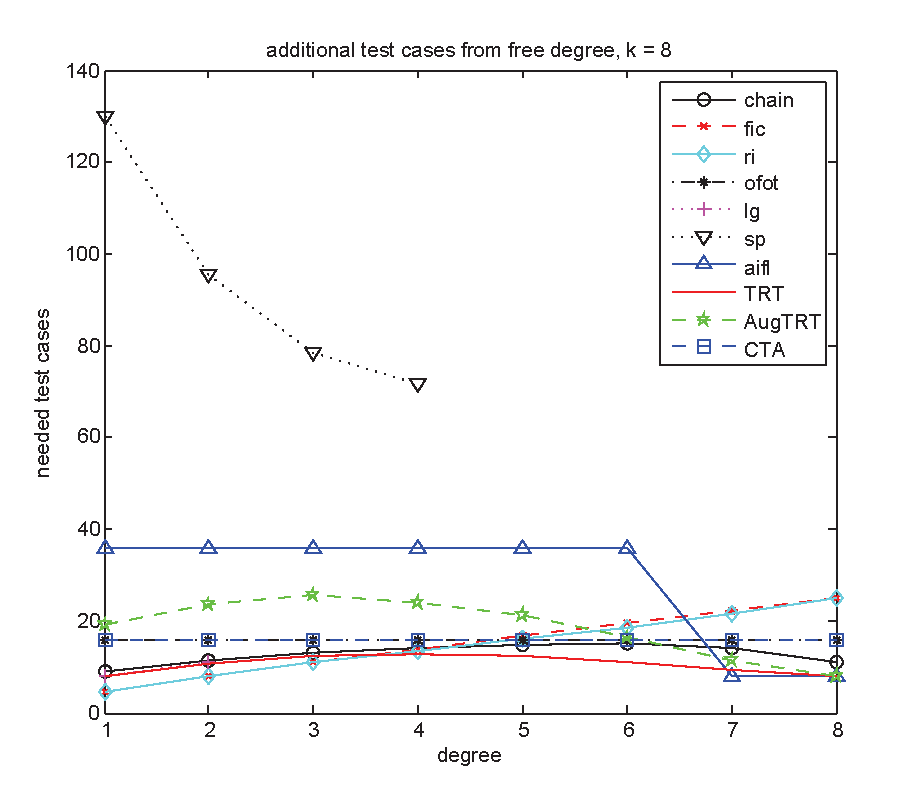
\includegraphics[width=2.8in]{freeD.eps}
 \caption{k = 8, t is free,single, additional test suites}
 \label{fig_free_d}
\end{figure}

we will enlarge some of them to figure \ref{fig_free_d_small}

\begin{figure}
 \centering
 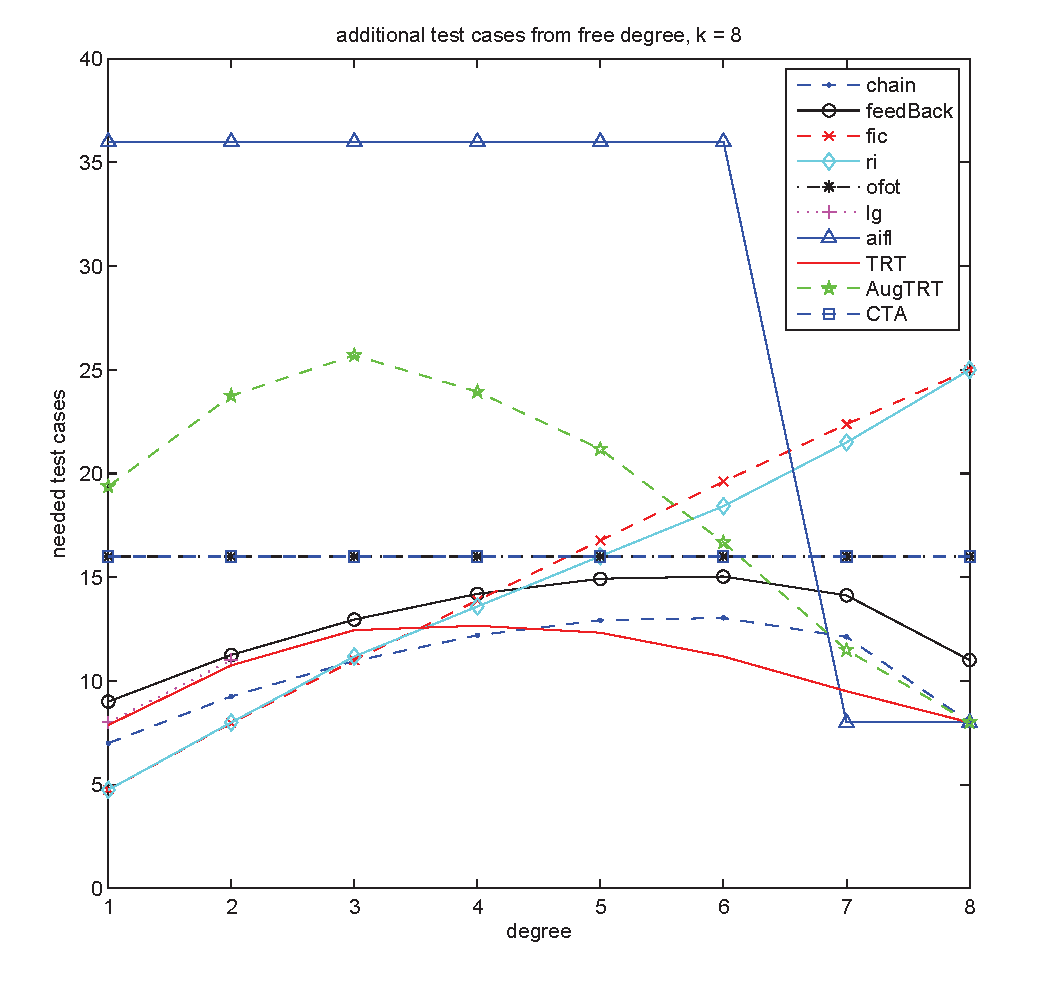
\includegraphics[width=2.8in]{freeD2.eps}
 \caption{k = 8, t is free,single, additional test suites for some algorithms}
 \label{fig_free_d_small}
\end{figure}


\section{Empirical Case study}\label{sec:realEx}
 While we got know that our approach have a better performance than others in several scenarios such as a failing test case contains multiple MFSs, the generated extra test case introduces newly MFS and so on from previous simulated experiments, it did not give us strong confidence in that our approach will also perform well in real software systems. One important reason of this is that we don't know whether these competitive scenarios for our approach existed in real software systems. So to eliminate the doubt we conduct a series empirical studies in this section. These empirical studies aimed to answer the following questions:

 Q1:Is there any test case that contain multiple MFSs, and if so, do they overlapped each other? Do any of these MFSs have high degree and how likely does it introduce newly MFS when generate extra test cases.

 Q2:How well of these approaches mentioned in previous sections performed when identifying the MFS in the real softwares?

 Q3:If we combine the result of one approach with another one, does it give us a better result than both of them?

The subject systems for these studies are HSQLDB(2.0rc8). HSQLDB is a database management system written in pure java. All of them have millions of uncommented lines of code. And they all share the same proceedings depicted in Fig.\ref{proceeding} when tested in the following studies.
\begin{figure}
 \centering
 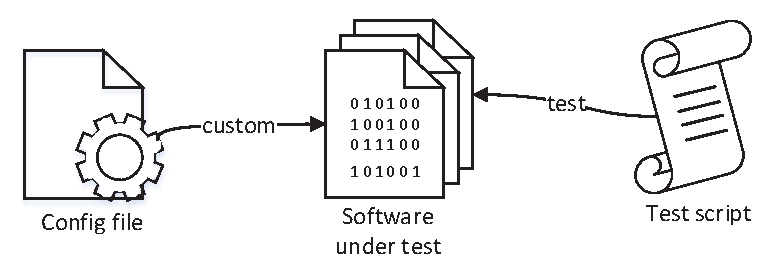
\includegraphics[width=2.7in]{proceed.eps}
 \caption{proceeding}
 \label{proceeding}
\end{figure}

As see from the figure, there are three modules in this proceeding: configuration file, software under test and the test script. The software under test is a set of software components which supply some interfaces, with which one can invoke the serving functions of the software. The configuration file is the file that can custom the properties of the software, and the test script is a executable file which test some functions of the software. In specific, the proceeding is trying different configuration of the software by changing the content of the configuration file, and then executing the same test script to observe the result.

\subsection{experimental setup}
Before we use these programs for study, we will take the following steps for each program to obtain the basic information of them, 1)Build the input configuration model of the subject program 2)execute the test case under each possible configuration and record their executed result. 3)list all the types of fault during testing and judge their priority.

We will depict these processes and results for each subject program in detail.
\subsubsection{HSQLDB}
Through searching the developers' community of HSQLDB in sourceforge, we found a buggy version with its faulty description in [], and a test script is attached which can reproduce the bug. The original test script only considered one option which have two values, remaining the other options set default values. To see what will happen when executing the test script under more different configurations, we need add some other options which may influence the behaviour of the database management software. From numerous optioins of HSQLDB, We chose some of the options that control the properties of table, some control the sql, some control the server and some control the result set. Along with the one in the original test script, we derive a input configuration model of HSQLDBlisted in table \ref{modelHSQLDB}.

\begin{table}\renewcommand{\arraystretch}{1.3}
  \caption{input model of HSQLDB} \centering
  \label{modelHSQLDB}
  \begin{tabular}{p{0.9\columnwidth}}\hline
  \hline
   \bfseries  SQL  properties(TRUE/FALSE)\\
    \hline
    sql.enforce\_strict\_size, sql.enforce\_names,sql.enforce\_refs, sql.enforce\_size, sql.enforce\_types, sql.enforce\_tdc\_delete, sql.enforce\_tdc\_update
  \end{tabular}

  \begin{tabular}{c*{2}{p{0.53\columnwidth}}}
  \hline
  \bfseries table properties &   \bfseries values \\
   \hline
   hsqldb.default\_table\_type & CACHED, MEMORY\\
   hsqldb.tx & LOCKS, MVLOCKS, MVCC\\
   hsqldb.tx\_level & read\_commited, SERIALIZABLE\\
   hsqldb.tx\_level & read\_commited, SERIALIZABLE
  \end{tabular}

  \begin{tabular}{c*{2}{p{0.53\columnwidth}}}
  \hline
  \bfseries Server properties &   \bfseries values \\
   \hline
   Server Type & SERVER, WEBSERVER, INPROCESS \\
    existed form & MEM, FILE
  \end{tabular}

  \begin{tabular}{c*{2}{p{0.53\columnwidth}}}
  \hline
  \bfseries Result Set properties &   \bfseries values \\
   \hline
    resultSetTypes & TYPE\_FORWARD\_ONLY,TYPE\_SCROLL\_INSENSITIVE, TYPE\_SCROLL\_SENSITIVE\\\
    resultSetConcurrencys & CONCUR\_READ\_ONLY,CONCUR\_UPDATABLE \\
    resultSetHoldabilitys & HOLD\_CURSORS\_OVER\_COMMIT, CLOSE\_CURSORS\_AT\_COMMIT
  \end{tabular}

  \begin{tabular}{c*{2}{p{0.53\columnwidth}}}
  \hline
  \bfseries option in test script &   \bfseries values\\
   \hline
   StatementType & STATEMENT, PREPAREDSTATEMENT
  \end{tabular}

\end{table}

%execute
We denoted this input model as ($2^{13}, 3^3$). There are $ 2^{13} * 3 ^ 3 = 221184 $ possible configurations in total. We executed the test script under each of the 221184 configurations and recorded their result. In specific, there are 147472 configurations triggered exceptions, while others passed this test. These exceptions can be classified to 4 types according to the exception traces. Through viewing the exception trace info and the source code of test script, we sorted out the priorities of these exceptions. Table \ref{faultyPriority} shows the detail of the 4 types of exceptions. The "exception ID" column shows the id of the exception. The "lower priority "column gives the IDs of exception which have lower priority than this exception. The "num of configs" means the number of test configurations under which the test script triggered this type of exception when executing.

%faulty type and their priority
\begin{table}\renewcommand{\arraystretch}{1.3}
  \caption{faulty and Priority} \centering
  \label{faultyPriority}

  \begin{tabular}{c*{3}{p{0.33\columnwidth}}}
  \hline
  \bfseries exception\ ID  &   \bfseries lower\ priority & \bfseries num\ of\ configs\\
   \hline
   1 & 2 & 36855\\
   2 & 1 & 110558\\
   3 & 1 2 & 58\\
   4 & 1 2 & 1
  \end{tabular}

\end{table}


\subsection{Study 1: what the schemas like in practice}
In the first study, we aimed to answer the Q1. We need to investigate the MFSs of the real softwares to see 1) Do there existed multiple MFSs in the same configuration? 2) if so, how many of them overlapped each other? 3) Do any of the MFSs have the degree larger than 2. 4) What the possibility of introducing newly MFSs when generating extra configurations. In particular we will inspect the MFSs in HSQLDB.

The first obstacle of case study 1 is that we don't know the MFSs in the real softwares. The original bug report page of these softwares[][] can give us hints of the MFSs of the software, but it is not enough for us to get accurate MFSs of the software. The reason is that we had added more options to test the script which resulted in more exceptions than reported and the original reported exception can also be related to more options that didn't be mentioned in the bug report.

So the only way to recognize the MFSs in the software is searching all the schemas in a configuration one by one, and then judging the state of the schema according to the definition and propositions. We will repeat the process in all the possible configurations of the software, this process is time-assuming which can be optimized by introducing hash table and adjusting the order when searching the schema of a configuration. We will omit these details as it is not point of this paper. Lastly after this time-assuming process we got the accurate MFSs for each software, we recorded them for later use.

\subsubsection{Measure the MFSs in the softwares}
As MFSs in the softwares are figured out, we can easily count the number of configurations contain multiples MFSs and MFSs that overlapped each other, as well as count the number of  MFSs that have a degree larger than 2.  But for the possibility of introducing newly MFSs when generating extra configuration (brief as possibility of introducing), we yet can't measure it for we didn't define how to compute the "possibility". We will give a formula to compute the possibility of introducing next, before then we will explain how is this formula derived.

First we should understand under which condition will the event of introducing newly MFSs harms our identifying algorithm.  Consider the following scenario.

For a test case of which we want to identify the MFS, say test case A,  if we change one factor of it to generate a new test case, say test Case B.  Then assume in this step we introduced a new failure-inducing schema, but meanwhile we didn't break the original failure-inducing schema in the test case A when we generate B, in other words, the MFS in A is still in B.

At this situation it will not influence our identifying result for that if we did not introduce the schema, our result is the same---trigger the same failure.

Consider another scenario, still for test case A, and we also change one factor of it to generate a new test case, say test Case C. Similarly, we introduced a new MFS, but different from the first scenario, this time we break the original MFS in the test case A when we generate C, which means the MFS in A is not in C.

At this situation it will influence our identifying result for that our expected result is that C should passed the test as we have broken the MFS in A. But the result failed at last. And we could owe this failure to some schema in A that is not the real MFS if we did nothing to deal with the introducing problem.

So we just need consider the possibility of the situation of simultaneously broking one MFS and introducing another MFS. This metric is related to the cost of changing one schema to another schema. The followed formula define the changing cost of two schemas:

ChangeCost(A, B) = $|T(A,B)| +\sum_{i \in T(B,A)}\left(P_{i} / 2\right) + \sum_{i \in S(A,B)}\left( |A_{i} - B_{i}| / 2\right)$

In this formula, A and B represent two different schemas. the denotation of T(A,B) gives the parameters in A but not in B. And S(A,B) means the parameters in both A and B, but their value is different.
$P_{i}$ refers to the number of values in the $i$th parameter of SUT, and $A_{i}$ is the value of one factor in Schema A , the factor is the $i$th parameter of SUT.

Then the introduce rate of a SUT is defined as:

$\dfrac {\sum_{a , b \in MFSs, a \neq b }\left(ChangeCost(a,b)\right)} {|MFSs|\times |MFSs - 1|}$

\subsubsection{result and analysis}
The statistic info of MFSs of the real software is listed in Table \ref{mfs-exp}.

\begin{table*}\renewcommand{\arraystretch}{1.3}
  \caption{MFSs information of each exception} \centering
  \label{mfs-exp}

  \begin{tabular}{c|c|c|c|c|c}
  \hline
  \bfseries exp\ ID  &  \bfseries MFSs & \bfseries degree\ than\ 2 & \bfseries mutliple\ MFSs& \bfseries overlapped\ MFSs &\bfseries intro rate\\
   \hline
   1 & 9 & 8 & 8 & 8 &0.1028\\
   2 & 24 & 23 & 25 & 1 &0.0145\\
   3 & 56 & 56 & 1 & 1 &0.0026\\
   4 & 1 & 1 & 0 & 0 & -
  \end{tabular}

\end{table*}

In this table,  "exp ID" is the id of exception which the MFSs will trigger, "MFSs" gives the number of MFSs that can trigger this type of Exception show in "exp ID" column. Column "degree than 2" list the number of MFSs that have a degree larger than 2.  "multiple MFSs" means the number of configurations that contain multiple MFSs. The column "overlapped MFSs" gives the number of configurations that contain MFSs that overlapped each other. And the last column "intro rate" shows the introduce possibility of newly MFSs when generating extra test configuration.

From this result, we will answer the sub-question of Case study 1 one by one.

1)Do there existed multiple MFSs in the same configuration?

Answer: yes. Although it is rare among the failing configurations(for exception 1, there are 36855 configurations trigger the same exception, and only 8 configurations contain multiple MFSs), but it do exist in the configurations of real software, we can see except the $4$th exception which just has one MFS, all the other exception have configurations have multiple MFSs, which are 8,25,1 respectively.

2)if so, how many of them overlapped each other?

Answer: most of them are overlapped each other. We learned configurations which have overlapped MFSs is 8, 1, 1 respectively. As we all know, the configurations have overlapped MFSs is just one part of the configurations have multiple configurations. Considering the configurations contain multiple MFSs is rare, which are 8 , 25, 1 respectively, then the  We think it is a high possibility when we encounter the situation that configurations contain multiple MFSs and these MFSs overlapped with each other.

One possible explanation for this phenomenon may be real softwares may have many branches, and these branches may have iteration, so for some MFSs , they may share the same entrance of the branch.

3)Do any of the MFSs have the degree larger than 2.

Answer: yes.  It is clearly that almost all the MFSs in the software have a degree than 2, except one MFS for exception 1 ( 8 among 9 MFSs have degrees larger than 2) and one MFS for exception 2( 23 among 24 MFSs have degrees larger than 2).

4)What the possibility of introducing newly MFSs when generating extra configurations?

Answer: the possibility varies from one to another.

We can learn from the table that the intro rate of exception 1 is 0.1028, which are the biggest than others, and the smallest is the exception 3, which is 0.0026. They differ markedly, so the possibility of introducing newly MFSs depends on the specific exception and may have big difference among each other.

\subsection{Study 2: how these algorithms behave when applied in real softwares}
The second study aims to answer the Q2. We will evaluate the performance of each algorithm in identifying the MFSs of the real softwares.
\subsubsection{Study setup}
To conduct this case study, We will feed one failing configuration to each algorithm and use them to identify the MFSs. Then we will compare the results get by each algorithm to the real MFSs in that configuration given in the study 1 respectively. The comparison metrics is similar to the simulated experiment, which consists of  the number of extra test configurations needed, the precise and the recall. To be fair, no other information is given to each algorithm except the feeded failing configuration. We will repeat this comparison for each failing configuration of a exception. At last we will report the average number of test configurations , precise and recall for each algorithm.

As we will take a large number of configurations to identify( 147472 for HSQLDB), this is too big compact to some algorithms, such as TRT, IterAIFL, they can't even accomplish the task. Some other algorithm can complete this task but with a huge time cost, such as SP, it will take weeks or even months to complete. We will omit these algorithms in our comparison to make this study available in a relative short time. As a result, we just choose ChainFeedBack , FIC, RI, OFOT, LG, CTA as our comparison algorithms.

 \subsubsection{result and analysis}

 \begin{table*}\renewcommand{\arraystretch}{1.3}
  \caption{comparison in real softwares} \centering
  \label{compare-casestudy}

  \begin{tabular}{c|c|c|c|c}
  \hline
  \bfseries exp\ ID& \bfseries  algorithm   & \bfseries num\ of\ extra\ configs & \bfseries recall & \bfseries precise\\
   \hline
  1 & ChainFeedBack & 15.061 & 1.0 & 0.9995\\
  \  & FIC  &9.023& 0.9991 & 0.9988 \\
  \ & RI & 9.024 & 0.9991 & 0.9988 \\
  \  & OFOT &19.007 & 0.9997 & 0.9995 \\
  \  & LG &11.000 & 0.0 & 0.0\\
  \  & CTA &19.0 & 0.9997 & 0.9995\\
  \hline
  2 & ChainFeedBack & 13.058 & 0.9999 & 0.9996\\
  \  & FIC  &6.0160& 0.9999 & 0.9997 \\
  \ & RI & 6.0161 & 0.9999 & 0.9997 \\
  \ & OFOT &19.0 & 0.9997 & 0.9997 \\
  \  & LG &11.0005 & 0.9998 & 1.0\\
  \  & CTA &19.0 & 0.9997 & -\\
  \hline
  3 & ChainFeedBack & 19.793 & 0.9827 & 0.9827\\
  \  & FIC  &61.6551& 0.8879 & 0.89655 \\
  \ & RI & 62.6206 & 0.9396 & 0.9482 \\
  \ & OFOT &19.0 & 0.9827 & 0.9827 \\
  \  & LG &5.3448& 0 & -\\
  \  & CTA &19.0 & 0.9137 & 0.9137\\
  \hline
  4 & ChainFeedBack & 19.0 & 1.0 & 1.0\\
  \  & FIC  &65.0& 1.0 & 1.0 \\
  \ & RI & 65.0 & 1.0 & 1.0 \\
  \ & OFOT &19.0 & 1.0 & 1.0 \\
  \  & LG &5.0 & 0.0 & -\\
  \  & CTA &19.0 &1.0 & 1.0
  \end{tabular}
\end{table*}

 The result is shown in table \ref{compare-casestudy}. In this table, Column "exp\ ID" still means the ID for the specific exception. Column "algorithm" gives the specific algorithm measured in this row. Column "num of extra configs" shows the average number of extra configurations needed to generate to identify the MFSs. Column "recall" and "precise" respectively shows the average recall and precise which have been defined in the simulated experiment for each algorithm.

 We will discuss the result by column:

 1)the number of extra configurations: We may get two points in this column: a. no algorithms always need the smallest configurations in all conditions. For example,FIC needs the smallest configurations for exception 1(9.023) and exception 2(6.016) but needs the largest number of configurations for exception 4(65.0) as FIC may need a high cost dealing high way degree schema.  RI performs good at exception 2(6.016), but performs bad at exception 3(62.62) and 4 (65.0).  LG needs the smallest number of configurations for exception 3(5.344) and exception 4(5.0), but for exception 1 and 2 it doesn't perform as good as FIC and RI.  b. OFOT and CTA performs almost the same for all the exception exceptions(almost as 19.0, exception the OFOT for the exception 1(19.0007)), this is because they are not the adaptive method, they just change one factor one time for all the conditions. And the unique different is that OFOT add some more configurations to deal the introduce problem. c. Our algorithms performs moderately, better than OFOT for exception 1 and 2 but worse than others, and better than FIC and RI for exception 3 and 4 and worse than others. This is because our algorithm consider more conditions such as introduce, overlapped and high degree problem.

 2)recall : our algorithms perform the best in all the circumstances for this metric, which means our algorithms can find more MFSs than others algorithms when identifying the MFSs in a failing configuration. The reason why our approach have advantages over others is that we consider more scenarios when fed a failing configurations, especially we took account of the case multiple , overlapped MFSs in a test configuration and the case when the MFSs have a high degree. Other approaches may consider some of them, but none of them consider all these scenarios. Another point that needed note is that for exception 1, 3 and 4, the recall of LG algorithm is 0, it is a signal that in this three circumstances, the MFSs in the SUT have degrees larger than 2.

 3)precise : algorithm OFOT and our approach performs better than others (our approach is litter weaker than OFOT for the exception 2, which ours is 0.9996, OFOT is 0.9997). As we have discussed before, the condition that introducing newly configurations when generating extra test configurations can make the identifying result incorrectly, so it is a nature idea that if the algorithm deal with the introducing newly MFSs, the algorithm can get a more accurate result than those approaches don't consider this scenario. The result data show in this table is coincide with this idea. We can also learn that the machine learning approach-- CTA can also get a well result (0.9995, - , 0.9137, 1.0, slightly weaker than OFOT and our approach) in this column. Although this approach didn't consider the introducing scenario, the nature of dealing noisy data in machine learning can give this approach a some relief from those bad affects.

 In addition, we can find some regular among the exceptions, i.e., for all the algorithms , the recall and precise is best in 4, second best in 2 , little worse in 1, the worst in 3. This is coincided with the intro rate, which means that the intro rate really have a influence for the performance in algorithms.

 Overall, the answer to Q2 is: Our algorithms preforms good at recall and precise, and moderately in num of extra configs. This is coincided with the result in simulated experiment.

 \subsection{Study 3: Is combination useful?}
 We can learn from the result in the second case study that none of these algorithms can be the best among all the scenarios. So a nature question is that can we combine the result of multiple algorithms to find a better result. In this study we will carry out some experiments to answer this question, i.e., the Q3.
 \subsubsection{Study setup}
 To utilize the result of each algorithm, we build a voting system. Thus, choose some algorithms and take a voting schedule: if the a schema is identified more than one algorithms, we take it as MFS, otherwise, we will discard it. We will vary the number of algorithms and adopt different combination of algorithms to observe the result. In specific we will take 2, 3, 4, 5 and 6 algorithms as the voters respectively. In addition, we will take all the combination of algorithms for a specific number. Take 2 for example we will choose ChainFeedBack and OFOT as a combination, ChainFeedBack and RI as another combination and so on. The total number combination of algorithms for a specific number $n$ is $\binom{6}{n}$.

 For each combination of algorithms, we will record the metric "recall" and "precise" of voting result. To measure if the voting system is useful, we compare this voting "recall" to the highest "recall" of the algorithm among the combination. The same comparison is also made to the "precise" metric. Note that the highest "recall" and the highest "precise" is not necessarily belong to the same algorithm in a combination. As a example, for the combination "OFOT" and "RI" for the exception 2. The highest value of "recall" is , which belongs to "OFOT". and the highest value of "precise" is, which is belong to the "RI".  And our voting result will compare to the recall "" and precise "" respectively.
 \subsubsection{result and analysis}
 The detail comparison result is listed is table \ref{case-study3}. In this table, "Column" means. the "+" signal. means a promotion over the highest . and the "-" signal means a decreasing of the highest.
 \begin{table*}\renewcommand{\arraystretch}{1.3}
  \caption{the combination of algorithms} \centering
  \label{case-study3}

  \begin{tabular}{c|c|c|c|c|c|c}
  \hline
   \ &  ChainFeedBack &   FIC   &  RI &  OFOT &  LG &  CTA\\
   \hline
   \bfseries ChainFeedBack & - & \textbackslash & \textbackslash & \textbackslash & \textbackslash & \textbackslash\\
   \bfseries FIC  & \textbackslash & - & \textbackslash & \textbackslash & \textbackslash & \textbackslash\\
   \bfseries  RI  & \textbackslash & \textbackslash & - & \textbackslash & \textbackslash & \textbackslash\\
   \bfseries OFOT  & \textbackslash & \textbackslash & \textbackslash & - & \textbackslash & \textbackslash\\
   \bfseries LG  & \textbackslash & \textbackslash & \textbackslash & \textbackslash & - & \textbackslash\\
   \bfseries CTA  & \textbackslash & \textbackslash & \textbackslash & \textbackslash & \textbackslash & -
  \end{tabular}
\end{table*}

The answer to Q3 is that: yes, it has promotion, but very little.

\subsection{threats to validate}
how seeded bugs are representative
auto oracle, if we don't have a correct version, or we can't determine a test case is faulty and wrong, then what can i do?
timing result
One worrying aspect of this research is that it seems to consider only the number of tests and number of faults uncovered. In the practice of testing, it is as important or more important to know testing times.
\section{Related works and Discuss}\label{sec:related}
Detail list the history. In the experiment section, we just give some brief introduction.

Nie's approach in [3] and [6] first separates the faulty-possible tuples and healthy-possible tuples into two sets. Subsequently, by changing a parameter value at a time of the original test configuration, this approach generates extra test configurations. After executing the configurations, the approach converges by reducing the number of tuples in the faulty-possible sets.
Delta debugging [5] proposed by Zeller is an adaptive divide-and-conquer approach to locating interaction fault. It is very efficient and has been applied to real software environment. Zhang et al. [4] also proposed a similar approach that can identify the failure-inducing combinations that has no overlapped part efficiently,
Colbourn and McClary [7] proposed a non-adaptive method. Their approach extends the covering array to the locating array to detect and locate interaction faults.
C. Martiez [8-9] proposed two adaptive algorithms. The first one needs safe value as their assumption and the second one remove the assumption when the number of values of each parameter is equal to 2. Their algorithms focus on identifying the faulty tuples that have no more than 2 parameters.
Ghandehari.etc [10] defines the suspiciousness of tuple and suspiciousness of the environment of a tuple. Based on this, they rank the possible tuples and generate the test cases. Although their approach imposes minimal assumption, it does not ensure that the tuples ranked in the top are the faulty tuples.
Yilmaz [11] proposed a machine learning method to identify inducing combinations from a combinatorial testing set. They construct a classified tree to analyze the covering arrays and detect potential faulty combinations. Beside this, Fouch?[12] and Shakya [13] made some improvements in identifying failure-inducing combinations based on Yilmaz' work.

We list a comprehensive detail and comparison table \ref{comparison-metrics}as followed.

\begin{table*}\renewcommand{\arraystretch}{1.3}
  \caption{The comparison of each algorithms} \centering
  \label{comparison-metrics}
  \begin{tabular}{c|c|c|c|c|c|c}\hline
  \hline
  \bfseries algorithms & \bfseries time complexity  & \bfseries space complexity & \bfseries multiple schemas & \bfseries strength of schema & \bfseries safe value & \bfseries result style \\
  \hline
    CMINFS & O(log(n)) & O(n) & yes, no limit, can overlapped & 1~n & can handle & precise \\
  \hline
    FIC & O(log(n)) & O(n) & yes, no limit, can't overlapped & 1~n & can't handle & precise \\
    TRT & O(log(n)) & O($2^n$) & yes, no limit, can overlapped & 1~n & can handle &precise \\
    Spetrum & O(n*t) & O($n*t$) & yes, no limit, can overlapped & 1~n & can handle & a rank of possible \\
  \hline
  \end{tabular}

\end{table*}

But even we get the failure-inducing schemas, it is still having a gap to fetch the failure causing root from the code. Such as int the TCAS, we get the failure-inducing schemas, and this is caused by a code mutation in the code such as followed:.  So in the future, we will analysis the relationship between the failure-inducing schemas and the real code causing.


\section{Conclusion}\label{sec:conclusion}
The conclusion goes here.





% if have a single appendix:
%\appendix[Proof of the Zonklar Equations]
% or
%\appendix  % for no appendix heading
% do not use \section anymore after \appendix, only \section*
% is possibly needed

% use appendices with more than one appendix
% then use \section to start each appendix
% you must declare a \section before using any
% \subsection or using \label (\appendices by itself
% starts a section numbered zero.)
%


\appendices
\section{Proof of the First Zonklar Equation}
Appendix one text goes here.

% you can choose not to have a title for an appendix
% if you want by leaving the argument blank
\section{}
Appendix two text goes here.

The procedure :

$mutant_a$

$mutant_r$

$is pending schema$

$makechain$


% use section* for acknowledgement
\ifCLASSOPTIONcompsoc
  % The Computer Society usually uses the plural form
  \section*{Acknowledgments}
\else
  % regular IEEE prefers the singular form
  \section*{Acknowledgment}
\fi


This work was supported by the National Natural Science Foundation of China (No. 61272079), the Research Fund for the Doctoral Program of Higher Education of China (No.20130091110032), the Science Fund for Creative Research Groups of the National Natural Science Foundation of China(No. 61321491), and the Major Program of National Natural Science Foundation of China (No. 91318301)

% Can use something like this to put references on a page
% by themselves when using endfloat and the captionsoff option.
\ifCLASSOPTIONcaptionsoff
  \newpage
\fi



% trigger a \newpage just before the given reference
% number - used to balance the columns on the last page
% adjust value as needed - may need to be readjusted if
% the document is modified later
%\IEEEtriggeratref{8}
% The "triggered" command can be changed if desired:
%\IEEEtriggercmd{\enlargethispage{-5in}}

% references section

% can use a bibliography generated by BibTeX as a .bbl file
% BibTeX documentation can be easily obtained at:
% http://www.ctan.org/tex-archive/biblio/bibtex/contrib/doc/
% The IEEEtran BibTeX style support page is at:
% http://www.michaelshell.org/tex/ieeetran/bibtex/
\bibliographystyle{IEEEtran}

\bibliography{sigproc}
%
% <OR> manually copy in the resultant .bbl file
% set second argument of \begin to the number of references
% (used to reserve space for the reference number labels box)
%\begin{thebibliography}{1}
%
%\bibitem{IEEEhowto:kopka}
%H.~Kopka and P.~W. Daly, \emph{A Guide to \LaTeX}, 3rd~ed.\hskip 1em plus
%  0.5em minus 0.4em\relax Harlow, England: Addison-Wesley, 1999.
%
%\end{thebibliography}

% biography section
%
% If you have an EPS/PDF photo (graphicx package needed) extra braces are
% needed around the contents of the optional argument to biography to prevent
% the LaTeX parser from getting confused when it sees the complicated
% \includegraphics command within an optional argument. (You could create
% your own custom macro containing the \includegraphics command to make things
% simpler here.)
%\begin{IEEEbiography}[{\includegraphics[width=1in,height=1.25in,clip,keepaspectratio]{mshell}}]{Michael Shell}
% or if you just want to reserve a space for a photo:

\begin{IEEEbiography}[{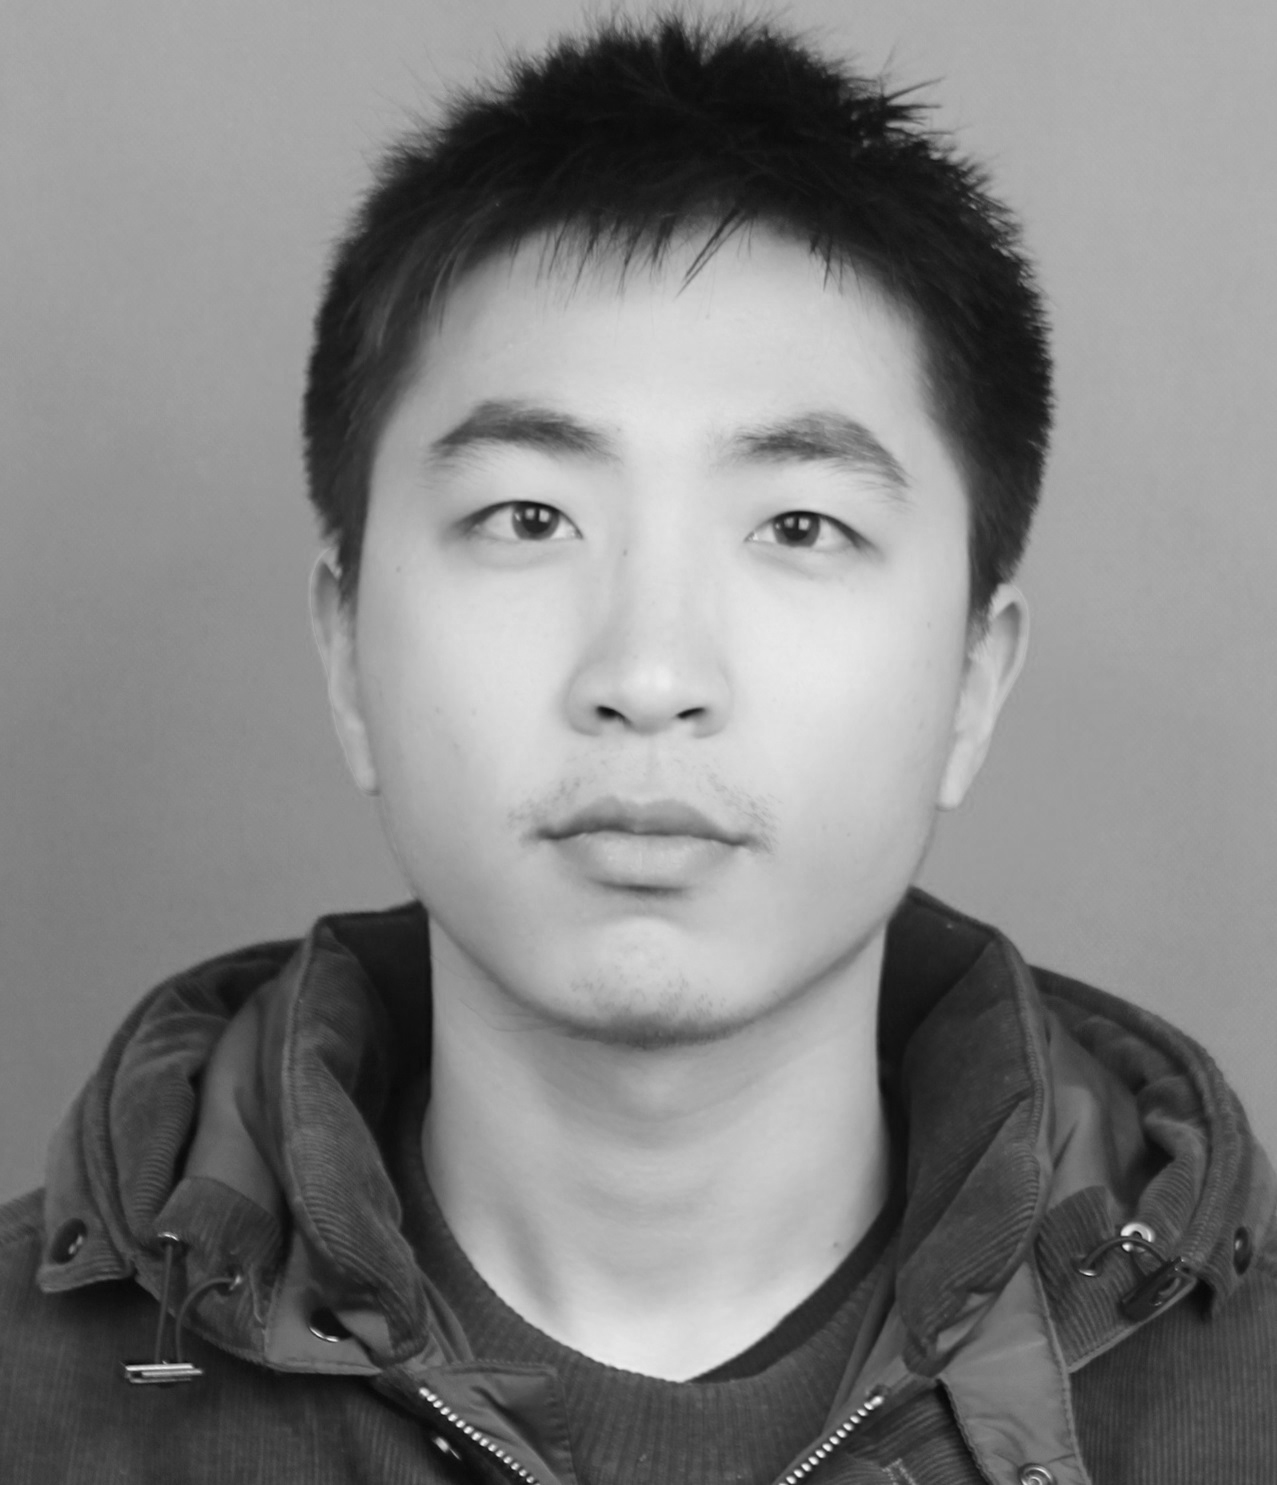
\includegraphics[width=1in,height=1.15in,clip,keepaspectratio]{niu}}]{Xintao Niu}
born in 1988, received his B.S degree from Nanjing University of Science and Technology. He is currently
working toward the PhD degree in the Department of Computer Science and Technology at
Nanjing University. His Research interest is software testing, especially on combinatorial testing and fault diagnosis. His work is supervised by Dr. Nie.
\end{IEEEbiography}

% if you will not have a photo at all:
\begin{IEEEbiography}[{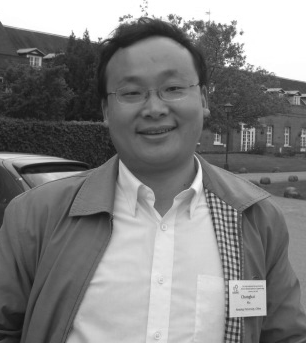
\includegraphics[width=1in,height=1.25in,clip,keepaspectratio]{nie}}]{Changhai Nie}
A Professor of Software Engineering in National Key Laboratory for Novel Software Technology and Department of Computer Science and Technology at Nanjing University. His research interest is software testing and search base software engineering, especially in combinatorial testing, search based software testing, software testing methods comparison and combination and et al.
\end{IEEEbiography}

\begin{IEEEbiography}[{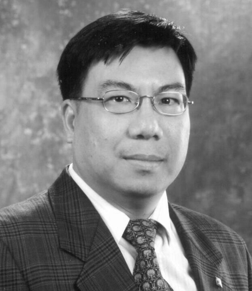
\includegraphics[width=1in,height=1.25in,clip,keepaspectratio]{hare}}]{Hareton Leung}
received the PhD degree in computer science from University of Alberta. He is an associate professor and the director at the Laboratory for Software Development and Management in the Department of Computing, the Hong Kong Polytechnic University. He currently serves on the editorial board of Software Quality Journal and Journal of the Association for Software Testing. His research interests include software testing, software maintenance, quality and process improvement, and software metrics
\end{IEEEbiography}

\begin{IEEEbiography}[{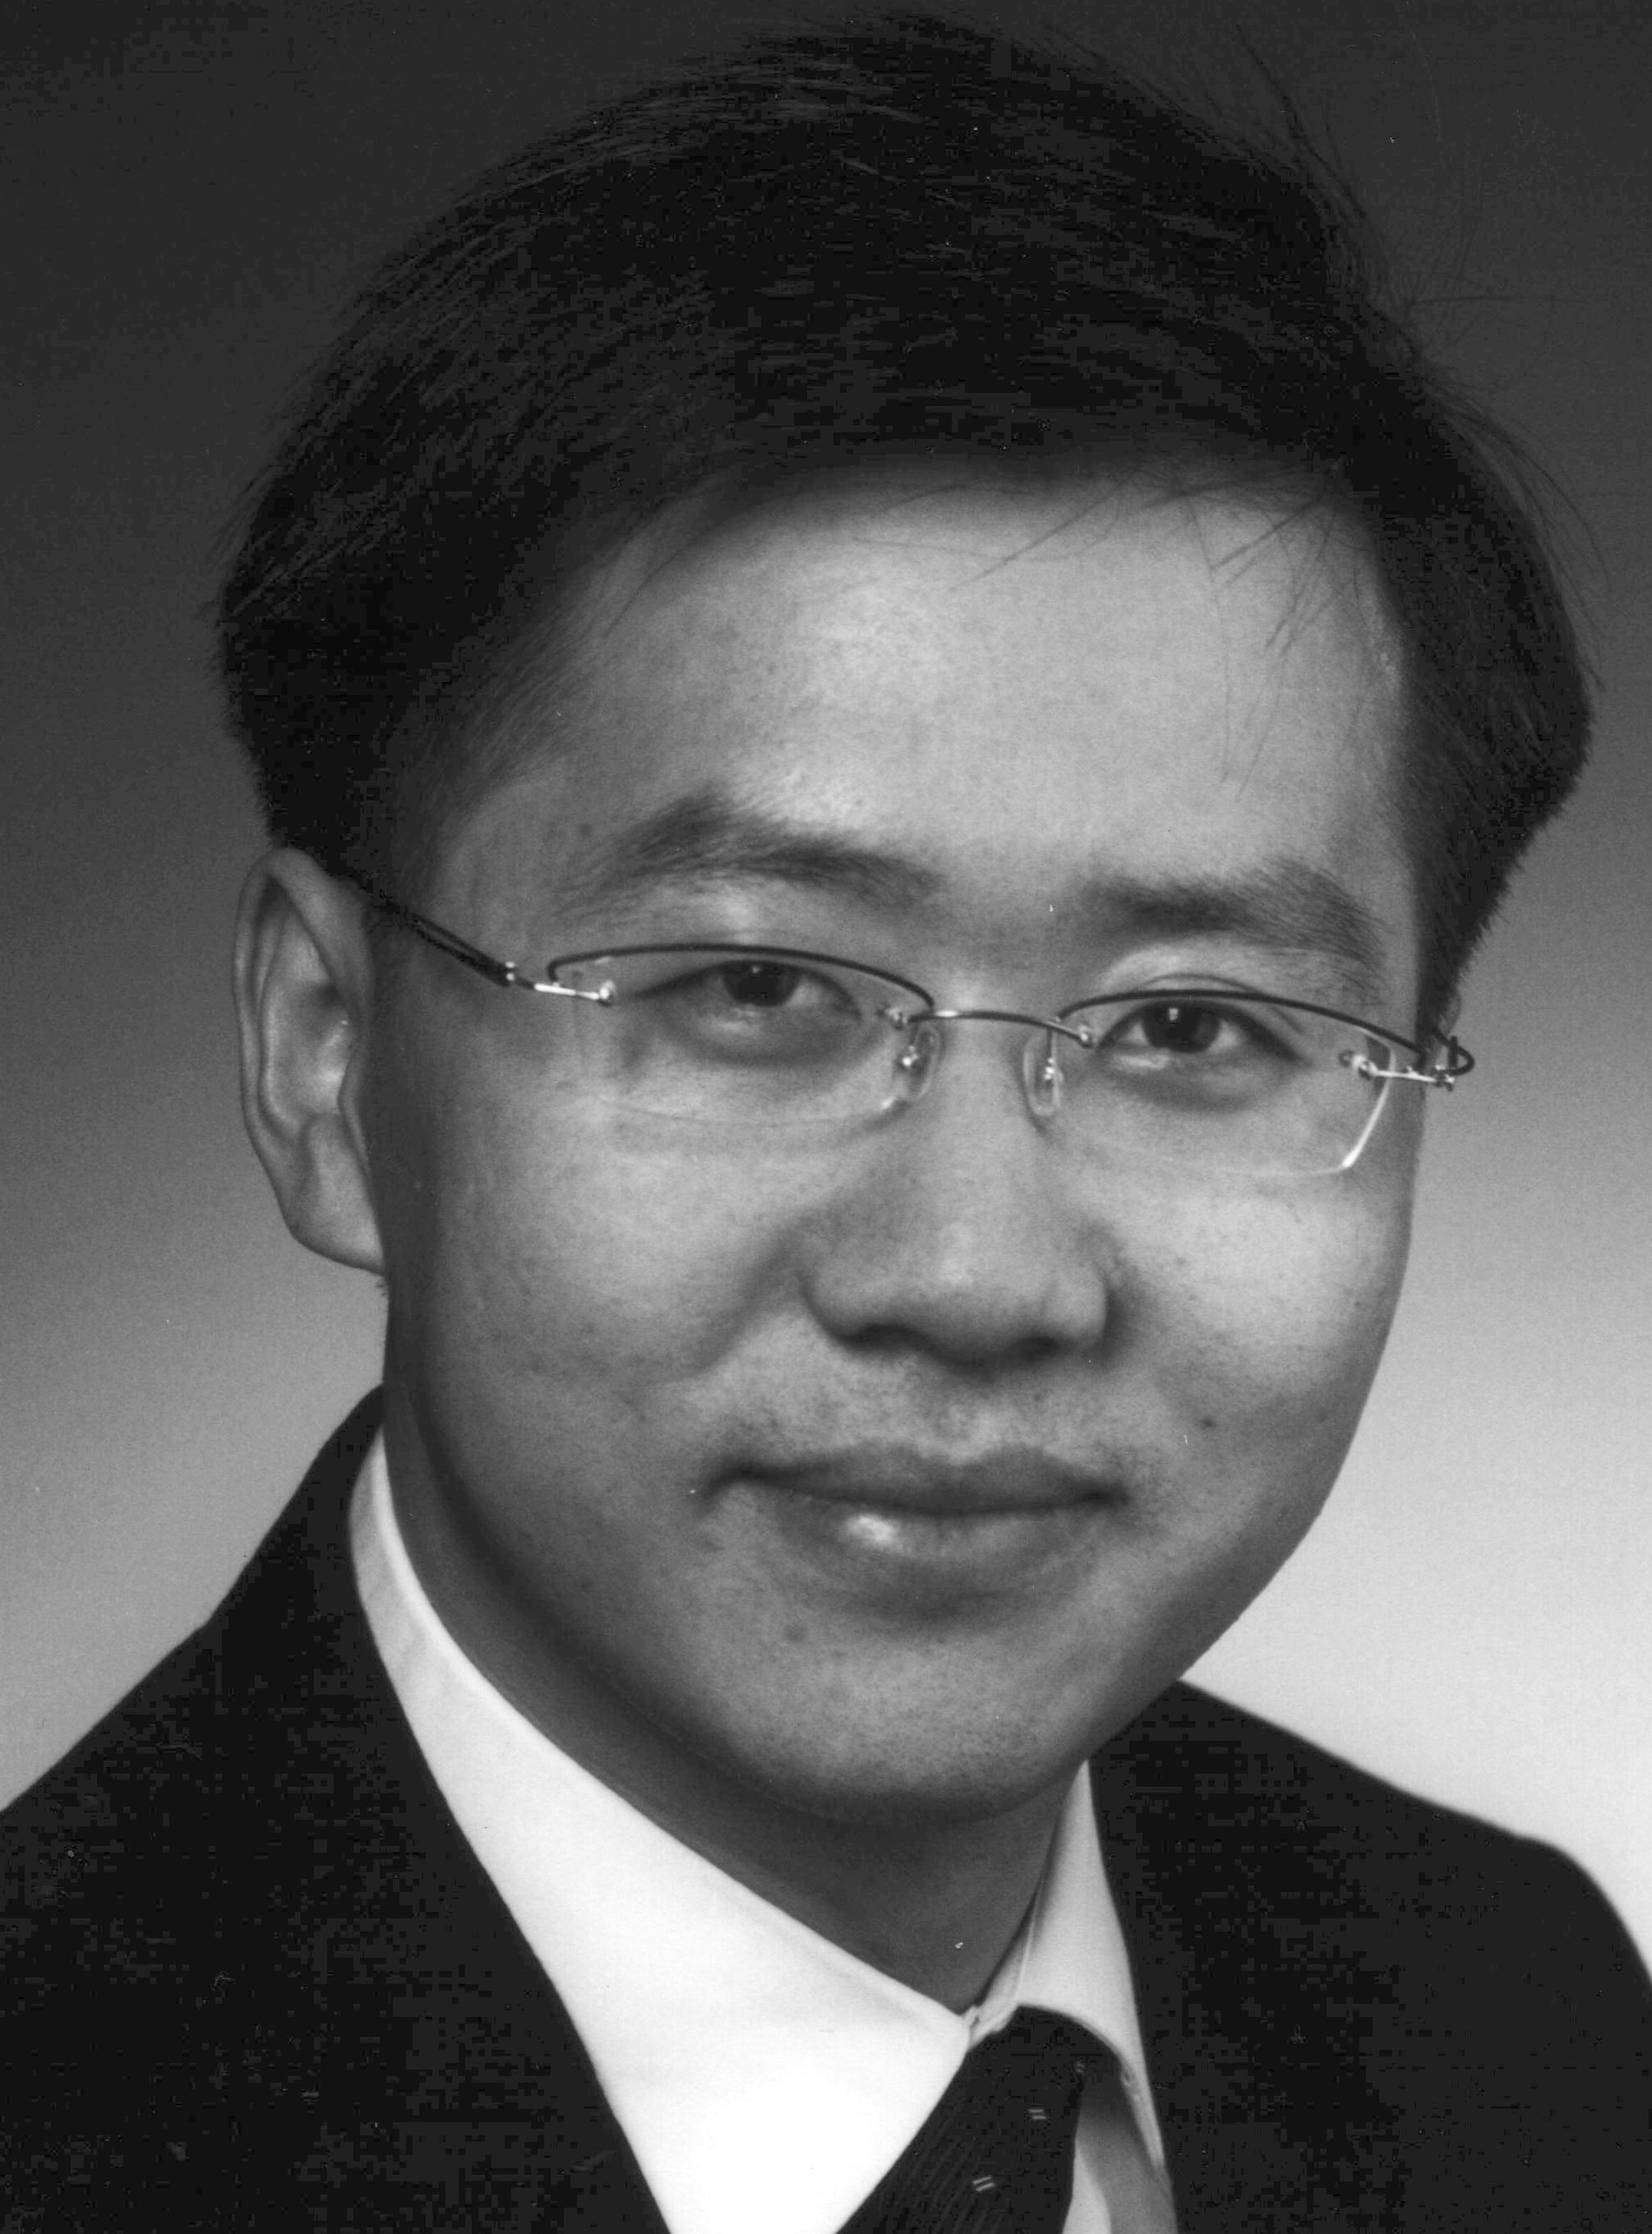
\includegraphics[width=1in,height=1.25in,clip,keepaspectratio]{lei}}]{Jeff Y. Lei}
is a full professor in Department of Computer Science and Engineering at the University of Texas, Arlington. He received his Bachelor's degree from Wuhan University (Special Class for Gifted Young), his Master's degree from Institute of Software, Chinese Academy of Sciences, and his PhD degree from North Carolina State University. He was a Member of Technical Staff in Fujitsu Network Communications, Inc. for about three years. His research is in the area of automated software analysis, testing and verification, with a special interest in software security assurance at the implementation level.
\end{IEEEbiography}

\begin{IEEEbiography}[{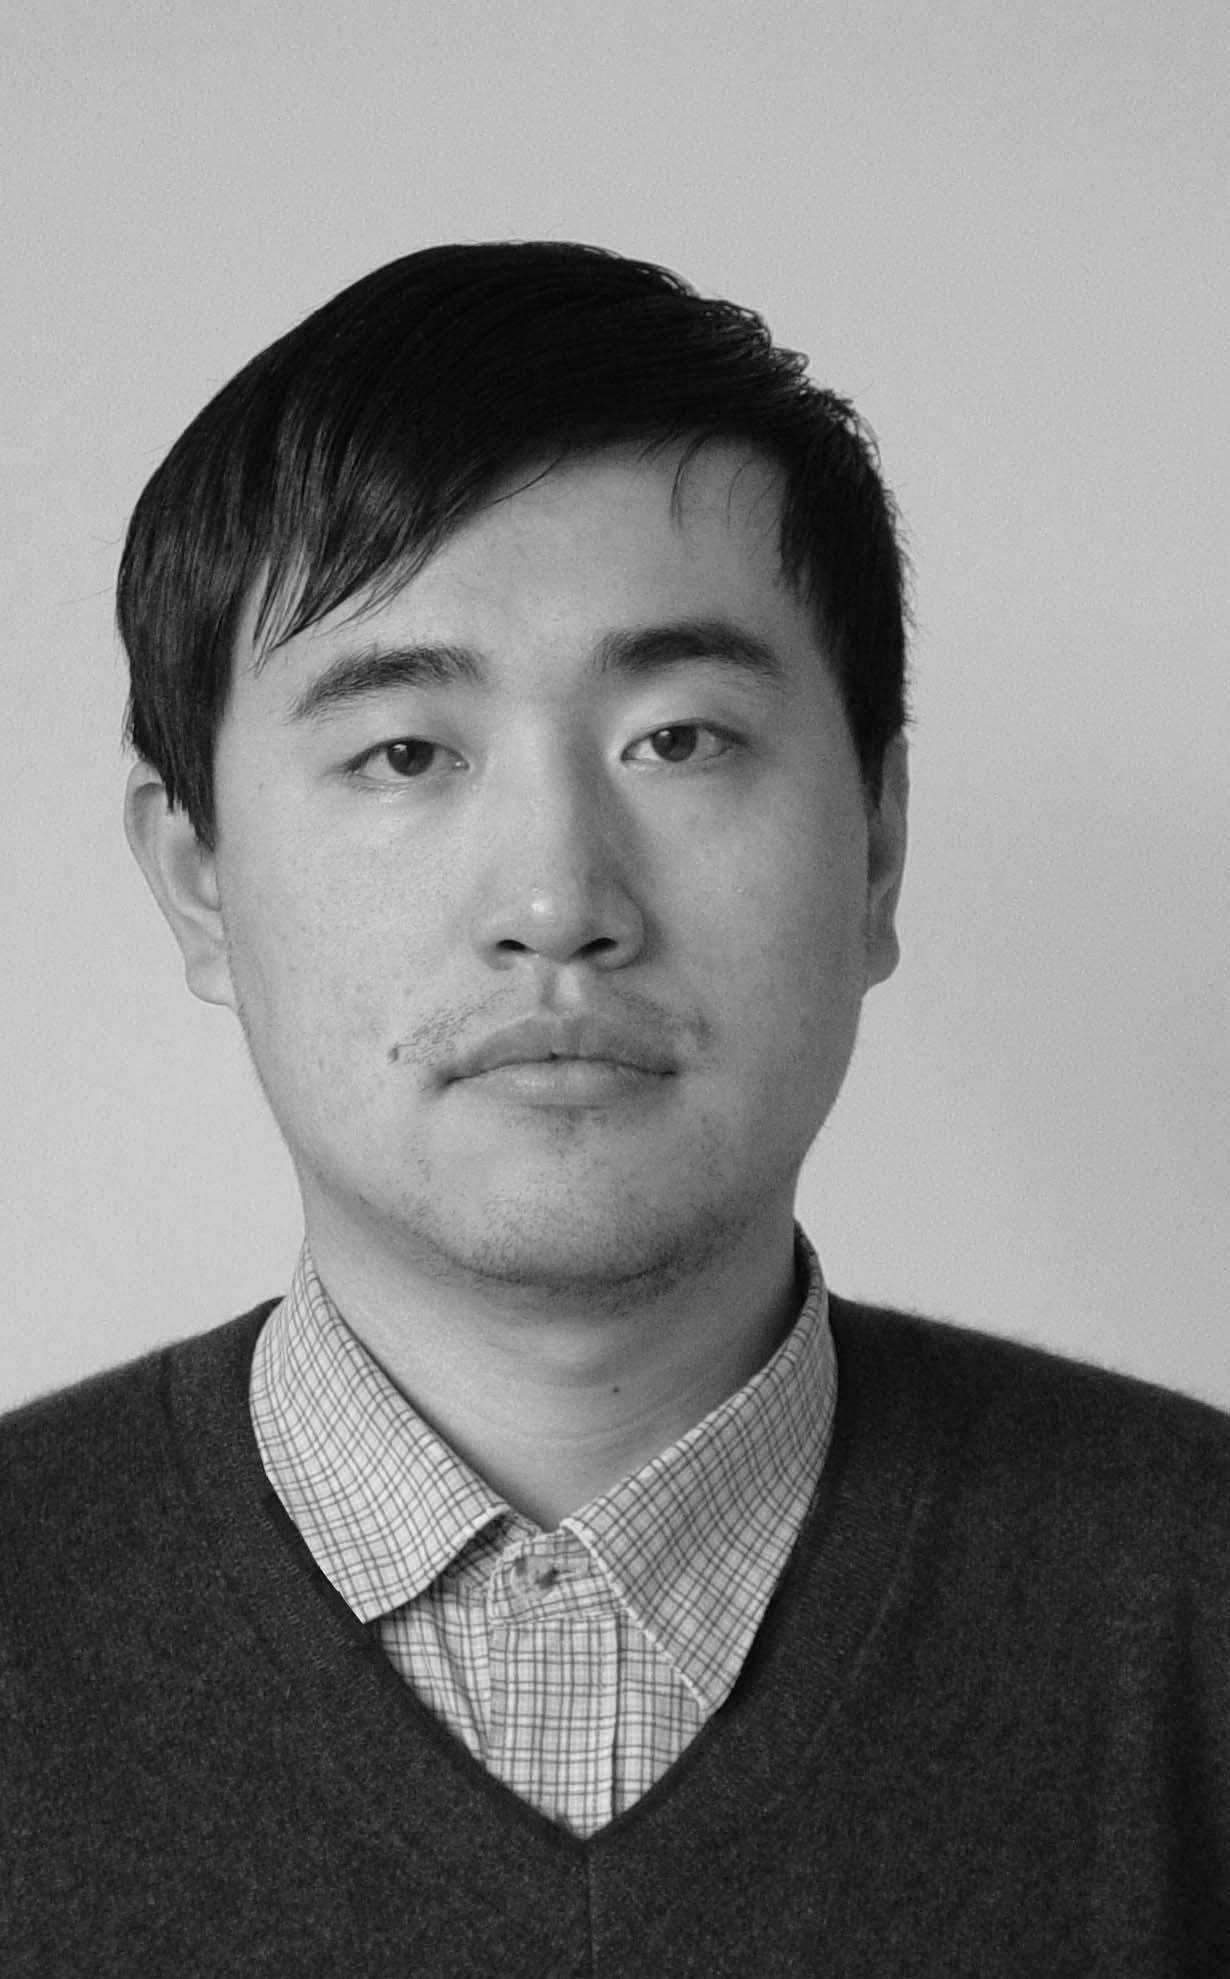
\includegraphics[width=1in,height=1.45in,clip,keepaspectratio]{xy}}]{Xiaoyin Wang}
born in Harbin, Heilongjiang Province, China in 1984. From September 2006 to January 2012, he was a Ph.D. candidate in the Software Engineering Institute (SEI) of Peking Univerisity. His advisor is Prof. Hong Mei, and he also did research under the supervision of Prof. Lu Zhang and Prof. Tao Xie. From Oct 2008 to Sept 2009, he visited Singapore Management University as a research fellow, where he worked with Prof. David Lo. In Jan. 2012, he began to work with Prof. Dawn Song, as a PostDoc in UC Berkeley. In August 2013, he joined the computer science department of University of Texas at San Antonio.
\end{IEEEbiography}
% You can push biographies down or up by placing
% a \vfill before or after them. The appropriate
% use of \vfill depends on what kind of text is
% on the last page and whether or not the columns
% are being equalized.

%\vfill

% Can be used to pull up biographies so that the bottom of the last one
% is flush with the other column.
%\enlargethispage{-5in}



% that's all folks
\end{document}



